%\documentclass[12pt,a4paper]{article}
\documentclass{elsarticle}
%\renewcommand{\baselinestretch}{1}

\usepackage[utf8]{inputenc}
\usepackage[english, russian]{babel}
\usepackage{amsmath, amsfonts, amssymb, amsthm}
\usepackage{pb-diagram} % Коммутативные диаграммы
\usepackage{graphicx, epsfig}
\usepackage{subfig}
\usepackage{hhline}
\usepackage{rotating}

%\graphicspath{ {figs/} }

% notations
% bold
\newcommand{\bz}{\mathbf{z}}
\newcommand{\bx}{\mathbf{x}}
\newcommand{\by}{\mathbf{y}}
\newcommand{\bw}{\mathbf{w}}
\newcommand{\bfx}{\mathbf{f}}
\newcommand{\bb}{\mathbf{b}}
\newcommand{\bu}{\mathbf{u}}
\newcommand{\bX}{\mathbf{X}}
\newcommand{\bZ}{\mathbf{Z}}
\newcommand{\bA}{\mathbf{A}}
\newcommand{\bI}{\mathbf{I}}
\newcommand{\bJ}{\mathbf{J}}
\newcommand{\bV}{\mathbf{V}}
\newcommand{\bU}{\mathbf{U}}
\newcommand{\bG}{\mathbf{G}}
\newcommand{\btheta}{\boldsymbol{\theta}}
\newcommand{\bPsi}{\boldsymbol{\Psi}}
\newcommand{\bpsi}{\boldsymbol{\psi}}
\newcommand{\bxi}{\boldsymbol{\xi}}
\newcommand{\bchi}{\boldsymbol{\chi}}
\newcommand{\bzeta}{\boldsymbol{\zeta}}
\newcommand{\blambda}{\boldsymbol{\lambda}}
\newcommand{\beps}{\boldsymbol{\varepsilon}}
\newcommand{\bZeta}{\boldsymbol{Z}}
% mathcal
\newcommand{\cX}{\mathcal{X}}
\newcommand{\cY}{\mathcal{Y}}
\newcommand{\cW}{\mathcal{W}}

\newcommand{\T}{^{\mathsf{T}}}

\newtheorem{theorem}{Теорема}%[section]
\newtheorem{df}{Определение}
\newtheorem{eq}{Пример}
\newtheorem{lemm}{Лемма}
\newtheorem{remark}{Замечание}

\begin{document}

\begin{frontmatter}

%% Title, authors and addresses

%% use the tnoteref command within \title for footnotes;
%% use the tnotetext command for theassociated footnote;
%% use the fnref command within \author or \address for footnotes;
%% use the fntext command for theassociated footnote;
%% use the corref command within \author for corresponding author footnotes;
%% use the cortext command for theassociated footnote;
%% use the ead command for the email address,
%% and the form \ead[url] for the home page:
%% \title{Title\tnoteref{label1}}
%% \tnotetext[label1]{}
%% \author{Name\corref{cor1}\fnref{label2}}
%% \ead{email address}
%% \ead[url]{home page}
%% \fntext[label2]{}
%% \cortext[cor1]{}
%% \address{Address\fnref{label3}}
%% \fntext[label3]{}

\title{Preference learning using partially ordered feature sets}

%% use optional labels to link authors explicitly to addresses:
%% \author[label1,label2]{}
%% \address[label1]{}
%% \address[label2]{}

\author{Mikhail Kuznetsov$^1$,Vadim Strijov$^2$}

\address{}

\begin{abstract}
%% Text of abstract

\end{abstract}

\begin{keyword}
%% keywords here, in the form: keyword \sep keyword

%% PACS codes here, in the form: \PACS code \sep code

%% MSC codes here, in the form: \MSC code \sep code
%% or \MSC[2008] code \sep code (2000 is the default)

\end{keyword}

\end{frontmatter}

\section{Введение}

Область обучения по предпочтениям~\cite{Fuernkranz2011} объединяет задачи машинного обучения с теорией группового выбора~\cite{kendall1938new, arrow19511963, kemeny1959mathematics} и агрегирования предпочтений для восстановления порядковой зависимости на множестве объектов с использованием линейных и порядковых экспертных оценок. В последние годы область обучения по предпочтениям приобрела особую актуальность в связи с возрастающей необходимостью решения задач информационного поиска~\cite{liu2009learning}, ранжирования, порядковой классификации и регрессии~\cite{mccullagh1980regression,herbrich1999large}, построения монотонных композиций алгоритмов~\cite{vorontsov1999local, hang2011short}.

%Первым типом задач является построение модели предпочтений на множестве объектов, заданных линейным признаковым описанием. Впервые задача в подобной постановке была рассмотрена для решения задачи информационного поиска~\cite{liu2009learning}. Требуется построить отображение множества объектов во множество действительных чисел, наиболее точно приближающее целевое отношение предпочтения. В задаче информационного поиска целевое отношение задается оценками асессоров на наборе документов, соответствующих запросу. Рассматривается класс линейных моделей и функция ошибки особого вида, штрафующая пары объектов, не согласованные по экспертно заданному отношению предпочтения. Моделями подобного типа являются модификация метода опорных векторов (RankSVM)~\cite{herbrich1999large, chen2009ranking} и модификация бустинга (RankBoost)~\cite{freund2003efficient}. В случае, когда целевое отношение предпочтения задается конечным набором меток, решается задача порядковой классификации и регрессии~\cite{Kotlowski2013}.

Рассматривается задача построения модели предпочтений на множестве объектов, заданных порядковым описанием. Задано множество объектов~$X$, на котором определено~$n$ отношений предпочтения~$z_1,...,z_n$, таких, что
\[
z_j(x_i,x_k)=[x_i\succeq_j x_k].
\]
Кроме того, на множестве объектов задано целевое отношение~$z_0$. Задача построения модели предпочтений заключается в построении отображения~$f:X\rightarrow Y$, где~$Y$~--- множество, наделенное отношением линейного порядка. При этом отношение предпочтения~$z_f$, построенное на основе отображения~$f$, должно минимизировать расхождение с целевым отношением~$z_0$, $S(z_f,z_0)\rightarrow \min$. 

Впервые задача в подобной постановке была рассмотрена в работе В.~Коэна и Р.~Шапиро~\cite{Cohen1999}. Для восстановления линейного порядка был предложен метод оценки матрицы попарного доминирования объектов. Основным требованием к отображению является монотонность по набору порядковых признаков~\cite{duivesteijn2008knn, Cheng2010}. Для решения этой задачи разработаны методы построения монотонных композиций алгоритмов, рассмотренные, например, в работах К.\,В.~Воронцова~\cite{vorontsov1999local}, а также в~\cite{Corrente2013}. Для соблюдения условий монотонности В.\,В.~Стрижовым был предложен подход на основе конусного представления предпочтений~\cite{strijov11utochnenie_zldm}, развиваемый в данной работе.

%Для достижения поставленных целей используется теория обучения по предпочтениям~\cite{Fuernkranz2011,Kaci2011}. Для исследования суперпозиции порядковых признаков используются механизмы теории голосования и общественного выбора, исследуемые в середине XX века К.~Эрроу~\cite{arrow19511963} и Дж.~Кемени~\cite{kemeny1959mathematics}, а также в более современных работах В.~Данилова~\cite{dan} и Д.~Саари~\cite{G.4/2008}. Для учета целевой переменной при восстановлении отношения предпочтения используются наработки в области обучения ранжированию~\cite{liu2009learning}, описанные в работах В.~Коэна и Р.~Шапиро~\cite{Cohen1999}. Исследуется обобщение задач порядковой регрессии~\cite{Corrente2013} и классификации~\cite{Kotlowski2013}, а также методы построения монотонных композиций, исследованные, в частности, в работах К.\,В.~Воронцова~\cite{vorontsov1999local,Spirin2011}. Для введения алгебраических структур, описывающих порядковый признак и частично упорядоченное множество, используется подход на основе конусов, впервые разработанный В.\,В.~Стрижовым~\cite{strijov11utochnenie_zldm}, а также теория анализа экспертной информации, исследуемая Б.\,Г.~Литваком~\cite{Litvak1982} и А.\,И.~Орловым~\cite{orlov2002expert}. Кроме того, используются элементы теории выпуклой оптимизации~\cite{StephenBoyd}, теории вероятностей, теории графов и теории важности критериев, разрабатываемой В.\,В.~Подиновским~\cite{podinovsky2007}.


%\paragraph{Наличие целевой переменной: обучение ранжированию.} В предыдущем параграфе были рассмотрены задачи теории общественного выбора и агрегирования предпочтений без учителя. В задачах подобного типа отсутствует целевое отношение предпочтения, или зависимая переменная, и основной целью является поиск ранжирования, являющегося средним в некотором смысле.

%Основной особенностью рассматриваемой задачи является необходимость учета целевого отношения предпочтения. Необходимость учета целевой переменной в задаче восстановления предпочтения появилась в конце XX века в связи с возникновением поисковых систем и появлением задачи~\emph{обучения ранжированию}~\cite{liu2009learning, hang2011short, burges2005learning}. Эта задача была впервые сформулирована в области информационного поиска и заключается в следующем. Поисковая система хранит внутри себя набор текстовых документов. На каждый запрос пользователя система возвращает список документов, отранжированный по степени релевантности, предсказанной системой. Помимо данных запрос-документ в системе также хранятся оценки асессоров, бинарные величины, указывающие, является ли документ релевантным запросу. Оценки асессоров являются обучающей информацией: параметры модели настраиваются таким образом, чтобы минимизировать расхождение между оценками асессоров и оценками релевантности, возвращаемыми системой.
%В качестве меры расхождения рассматриваются меры discounted cumulative gain (DCG) и normalized discounted cumulative gain (NDCG).

%Будет рассмотрено три важных примера отношений предпочтения, задаваемых отношениями частичного порядка:
%\begin{enumerate}
%\item Отношение предпочтения, заданное на целевой переменной~$y$. В этом случае, для набора объектов эксперты предоставляют информацию предпочтения на множестве значений их целевой переменной~$y_1\succeq y_2\succeq ...\succeq y_K$.
%\item Порядковое описание объектов~$x_i$. В этом случае, признаковое описание объекта предоставляется в порядковой шкале.
%\item Порядковые экспертные оценки весов признаков~$w$. Эксперты предоставляют информацию о том, какие показатели являются наиболее важными.
%\end{enumerate}

Основной трудностью для решения задач подобного типа является определение функции потерь~$S$ вследствие необходимости определения нормы на упорядоченном множестве~$Y$ и аппроксимации DCG-метрик~\cite{chen2009ranking}. В базовом случае эта функция является обратно пропорциональной функции порядковой корреляции~\cite{kendall1938new}. В~\cite{hang2011short} рассматривают три класса подходов к решению задачи обучению ранжированию, каждый из которых характеризуется особым видом функции потерь: поточечный (pointwise), попарный (pairwise) и списочный (listwise) подходы.

Поточечный подход к задачам обучения ранжированию~\cite{cossock2006subset, shashua2002ranking} основан на обобщении стандартных методов классификации и регрессии, при котором числовая ось значений отображения~$f$ разбивается на области, соответствующие упорядоченным меткам из множества~$Y$. Так, в~\cite{mccullagh1980regression} было предложено обобщение метода логистической регрессии, заключающееся в последовательном решении промежуточных задач бинарной классификации, различающих объекты смежных классов~$y_k,y_{k+1}$. Результирующий классификатор комбинирует результаты промежуточных. В дальнейшем такое представление задачи порядковой регрессии получило широкое развитие, в частности, в работах~\cite{Kotlowski2013, cardoso2007learning}.

В некоторых случаях,~\cite{Kotlowski2013, Spirin2011} в рамках поточечного подхода на промежуточном этапе решения задачи возникает подзадача монотонизации выборки, решаемая методами линейного программирования~\cite{StephenBoyd}. Задача заключается в поиске переменных~$p_i$, которые близки к значениям целевой переменной~$y_i$, но согласованы по монотонности с объектами~$x_i$:
\[
\arg\min_{p_i}(y_i-p_i)^2, \quad \text{при выполнении}~x_i \succeq x_j \Rightarrow p_i \geq p_j,
\]
где неравенство~$x_i \succeq x_j$ является покомпонентным.

В рамках попарного подхода задача ранжирования сводится к задаче двухклассовой классификации в пространстве пар объектов. Функция потерь штрафует пары объектов, не согласованных по экспертно заданному предпочтению~$z_0$. Одними из самых используемых алгоритмов для данного подхода служат модификация стандартного метода опорных векторов (RankSVM)~\cite{herbrich1999large, cao2006adapting} и модификация бустинга (RankBoost)~\cite{freund2003efficient}.

Методики обучения ранжированию в общем случае учитывают порядковую структуру зависимой переменной, но не учитывают порядковое описание объектов. Так, в рамках подхода RankSVM рассматриваются модели вида~$f(\bw,\bx)=\bw\T\bx$, то есть подразумевается, что объекты представлены линейным описанием~$\bx\in\mathbb{R}^n$. Тем временем, недавние исследования~\cite{duivesteijn2008knn, stenina2015ordinal} показали, что при порядковой структуре данных переход к монотонным моделям позволяет существенно повысить качество алгоритмов ранжирования.

Построение монотонного отображения~$f:X\rightarrow Y$ на декартовом произведении порядковых множеств~$X=X_1\times X_2\times \dots \times X_n$ в области обучения предпочтений получило название задачи порядковой классификации (регрессии) \emph{с~монотонными ограничениями}~\cite{Corrente2013, Kotlowski2013, dembczynski2008ordinal, Cheng2010}. Основная идея построения такого отображения заключается во введении дополнительного множества параметров, которые отвечают за преобразование порядковой~\cite{Moshkovich2002,Khurshid1993} шкалы множества~$X_j$, в линеаризации этого множества для поиска точки в линейном пространстве, наиболее согласованной с моделью~$f(\bw,\bx)$ в смысле функции потерь~$S$.


В последних работах~\cite{Fuernkranz2011} различные постановки задач с порядковой структурой описаний объектов и целевой переменной были объединены в область обучения по предпочтениям. Так, было рассмотрено три типа задач.
\begin{enumerate}
\item Ранжирование меток (англ.: label ranking), поиск отображения вида~$X\rightarrow S_Y$, где~$S_Y$~--- множество перестановок элементов~$Y$.
\item Ранжирование сущностей (англ.: instance ranking), поиск отображения~$X\rightarrow Y$, где~$Y$ является конечным множеством упорядоченных меток, $Y=\{y_1\succ ...\succ y_K\}$.
\item Ранжирование объектов (англ.: object ranking), поиск функции бинарного отношения на множестве объектов~$X$.
\end{enumerate}

%В данной работе также исследуется задача, объединяющая постановки~(\ref{constr:w})~и~(\ref{constr:y}) настоящего и предыдущего разделов. В частности, рассматриваются два конуса, соответствующие как экспертным оценкам целевой переменной, так и оценкам весов показателей. Предлагается процедура поиска согласованного решения~\cite{strijov11utochnenie_zldm} на основании минимизации расстояния между конусами.

В качестве частного случая, рассматривается задача порядковой классификации с монотонными ограничениями~\cite{Kotlowski2013, Corrente2013}, которая заключается в следующем: необходимо построить монотонную функцию, отображающую множество объектов во множество меток классов, причем на множестве меток классов введено отношение строгого линейного порядка. Требование монотонности функции определяется экспертными соображениями о влиянии того или иного фактора на модель. Постановка подобного типа возникает в задачах теории принятия решений, информационного поиска~\cite{Schafer2007,Trotman2005,Spirin2011}, обучения по предпочтениям~\cite{Fuernkranz2011}.
%
%Новизна предлагаемого в данном разделе решения задачи состоит в следующем: порядковое признаковое описание объектов задается набором отношений частичного порядка~\cite{Cheng2010}. Необходимо построить функцию, которая будет удовлетворять условию монотонности по каждому признаку.


\section{Задача восстановления предпочений}
%\paragraph{Основные определения.}
Задано \emph{множество объектов}~$X=\{x_1,...,x_m\}$ размера~$m$. Рассматриваемые объекты имеют порядковое признаковое описание: на~$X$ задано $n$~отношений предпочтения~$z_1,...,z_n$, каждое из которых описывает отношение доминирования между парами объектов,~$z_j(x_i,x_k)=[x_i\succeq_j x_k]$. Отношение предпочтения в общем случае является отношением частичного порядка, удовлетворяющего свойствам антисимметричности, рефлексивности и транзитивности.

На множестве объектов задано \emph{целевое отношение предпочтения}~$z_0=[x_i\succeq_0 x_k]$. Задача заключается в построении отображения~$f(x_i)\in \mathbb{R}$, удовлетворяющего двум основным условиям.
\begin{enumerate}
\item Монотонность по всем $z_1,...,z_n$,
\begin{equation}
x_i\succeq_1 x_k,~...,~x_i\succeq_n x_k\quad \rightarrow\quad f(x_i) \geq f(x_k).
\label{cond:MonFeat}
\end{equation}
\item Близость к целевому предпочтению~$z_0$:
\begin{equation}
S(X,f,z_0)~\rightarrow~\min.
\label{cond:ErrFnMin}
\end{equation}
\end{enumerate}
Условие близости к целевому отношению предпочтения выражается в виде минимизации некоторой функции ошибки~$S(X,f,z_0)$, штрафующей отклонение отношения~$z_f$, определяемого функцией~$f$, $z_f(x_i, x_k)=[f(x_i)\geq f(x_k)]$, от целевого отношения~$z_0$.

Каждому из отношений предпочтения~$z_j$ соответствует матрица предпочтений~$\bZ_j$, являющаяся матрицей инцидентности графа, соответствующего отношению~$z_j$.

%\begin{eq}
Приведем пример частично упорядоченного множества~$X$, состоящего из четырех объектов, таких что
\[
X=\{x_{1},x_{2},x_{3},x_{4}|~~z:x_{1}\succeq x_{2}, x_{2}\succeq x_{3}, x_{2}\succeq x_{4}\}.
\]
Отношение предпочтения~$z$ на объектах~$x_{1},x_{2},x_{3},x_{4}$ описывается графом частичного порядка с матрицей предпочтений~$\bZ$:
\[
\begin{diagram}
\node{x_{1}} \arrow[2]{e}{}
\node[2]{x_{2}} \arrow[2]{}
\arrow{se,b}{}
\node[2]{x_{3}} \\
\node[4]{x_{4}}
\end{diagram},
\quad
\bZ=
\begin{pmatrix}
1 & 1 & 1 & 1 \\
0 & 1 & 1 & 1 \\
0 & 0 & 1 & 0 \\
0 & 0 & 0 & 1 \\
\end{pmatrix}.
\]
\label{ex1}
%\end{eq}
%
%\paragraph{Постановка задачи.}
%На множестве~$X$ задано целевое отношение предпочтения~$z_0$, а также определена \emph{функция потерь} модели~$f$ на множестве объектов~$X$. Основной задачей является поиск отображения~$\hat{f}$, минимизирующего функцию потерь на~$X$,
%\[
%\hat{f}=\arg\min\limits_{f\in\mathcal{F}}S(f,X,z_0),
%\]
%где~$\mathcal{F}$~--- класс допустимых отображений.


\paragraph{Конусное описание предпочтений}
%\begin{df}
%Полиэдральный конус в~$\mathbb{R}^m$~--- это множество~$\mathcal{X}_0$, такое что
%\begin{equation}
%\mathcal{X}_0=\{\bchi\;|\;\bA\bchi\leq \mathbf{0},\;\bchi\in\mathbb{R}^m\},
%\label{df:Cone}
%\end{equation}
%для некоторой прямоугольной матрицы~$\bA$.
%\end{df}

Для построения модели введем определение конуса предпочтений, соответствующего множеству~$X$ с заданным на нем отношением предпочтения~$z$.
\begin{df}
Конусом предпочтений~$\cX$ для множества~$X$ с определенным на нем отношением частичного порядка~$z:~z=[x_i \succeq x_k]$ называется полиэдральный конус в пространстве~$\mathbb{R}^m_+$, сохраняющий порядок относительно~$z$:
\[
\cX=\{\bchi\in\mathbb{R}^m_+|\quad x_i\succeq x_k\rightarrow \chi_{i}\geq \chi_{k}\quad \forall~i,k=1,...,m\}.
\]
\label{df:ConePO}
\end{df}
Система неравенств, определяющая конус предпочтений~\eqref{df:ConePO}, задается матрицей~$\bA$:
\[
\mathcal{X}=\{\bchi\;|\;\bA\bchi\leq \mathbf{0},\;\bchi\in\mathbb{R}^m\}.
\]

Среди всех матриц~$\bA$ полиэдрального представления конуса~$\cX$ будем рассматривать прямоугольную матрицу размера~$m^2\times m$, где каждая строка соответствует паре элементов~$x_{i}, x_{k}$ и содержит максимум два ненулевых элемента:
\[
a_i=-1~\text{и}~a_k=1,~\text{если}~x_{i}\succeq x_{k}.
\]

\paragraph{Порождающее представление конуса}
Следующая теорема устанавливает вид порождающего представления конуса предпочтений: конус~$\cX^{\bZ}$, порождающие элементы которого являются столбцами матрицы предпочтений, является подмножеством конуса предпочтений~$\cX$.
\begin{theorem}
\label{thm:ConeSubset}
$\cX \supset \cX^{\bZ}=\{\bZ\blambda~|~\blambda \geq \mathbf{0}\}.$
\end{theorem}

%Согласно теореме Минковского-Вейла, каждый полиэдральный конус допускает представление через конечный набор порождающих~\cite{charnes1958strong}. Другими словами, полиэдральный конус~$\cX^A$ представим в виде
%\begin{equation}
%\cX^A=\{\bchi~|~\bchi=\sum\limits_{k=1}^{r}\lambda_{k}\bzeta_{k},~\lambda_{k}\geq 0\},
%\label{df:ConeGen}
%\end{equation}
%где~$\bzeta_{k}$~--- порождающий элемент конуса~$\cX^A$, а~$r$~--- число порождающих элементов. В общем случае, количество порождающих~$r$ зависит от структуры отношения частичного порядка множества~$X$.

\begin{figure}[h]
\begin{center}
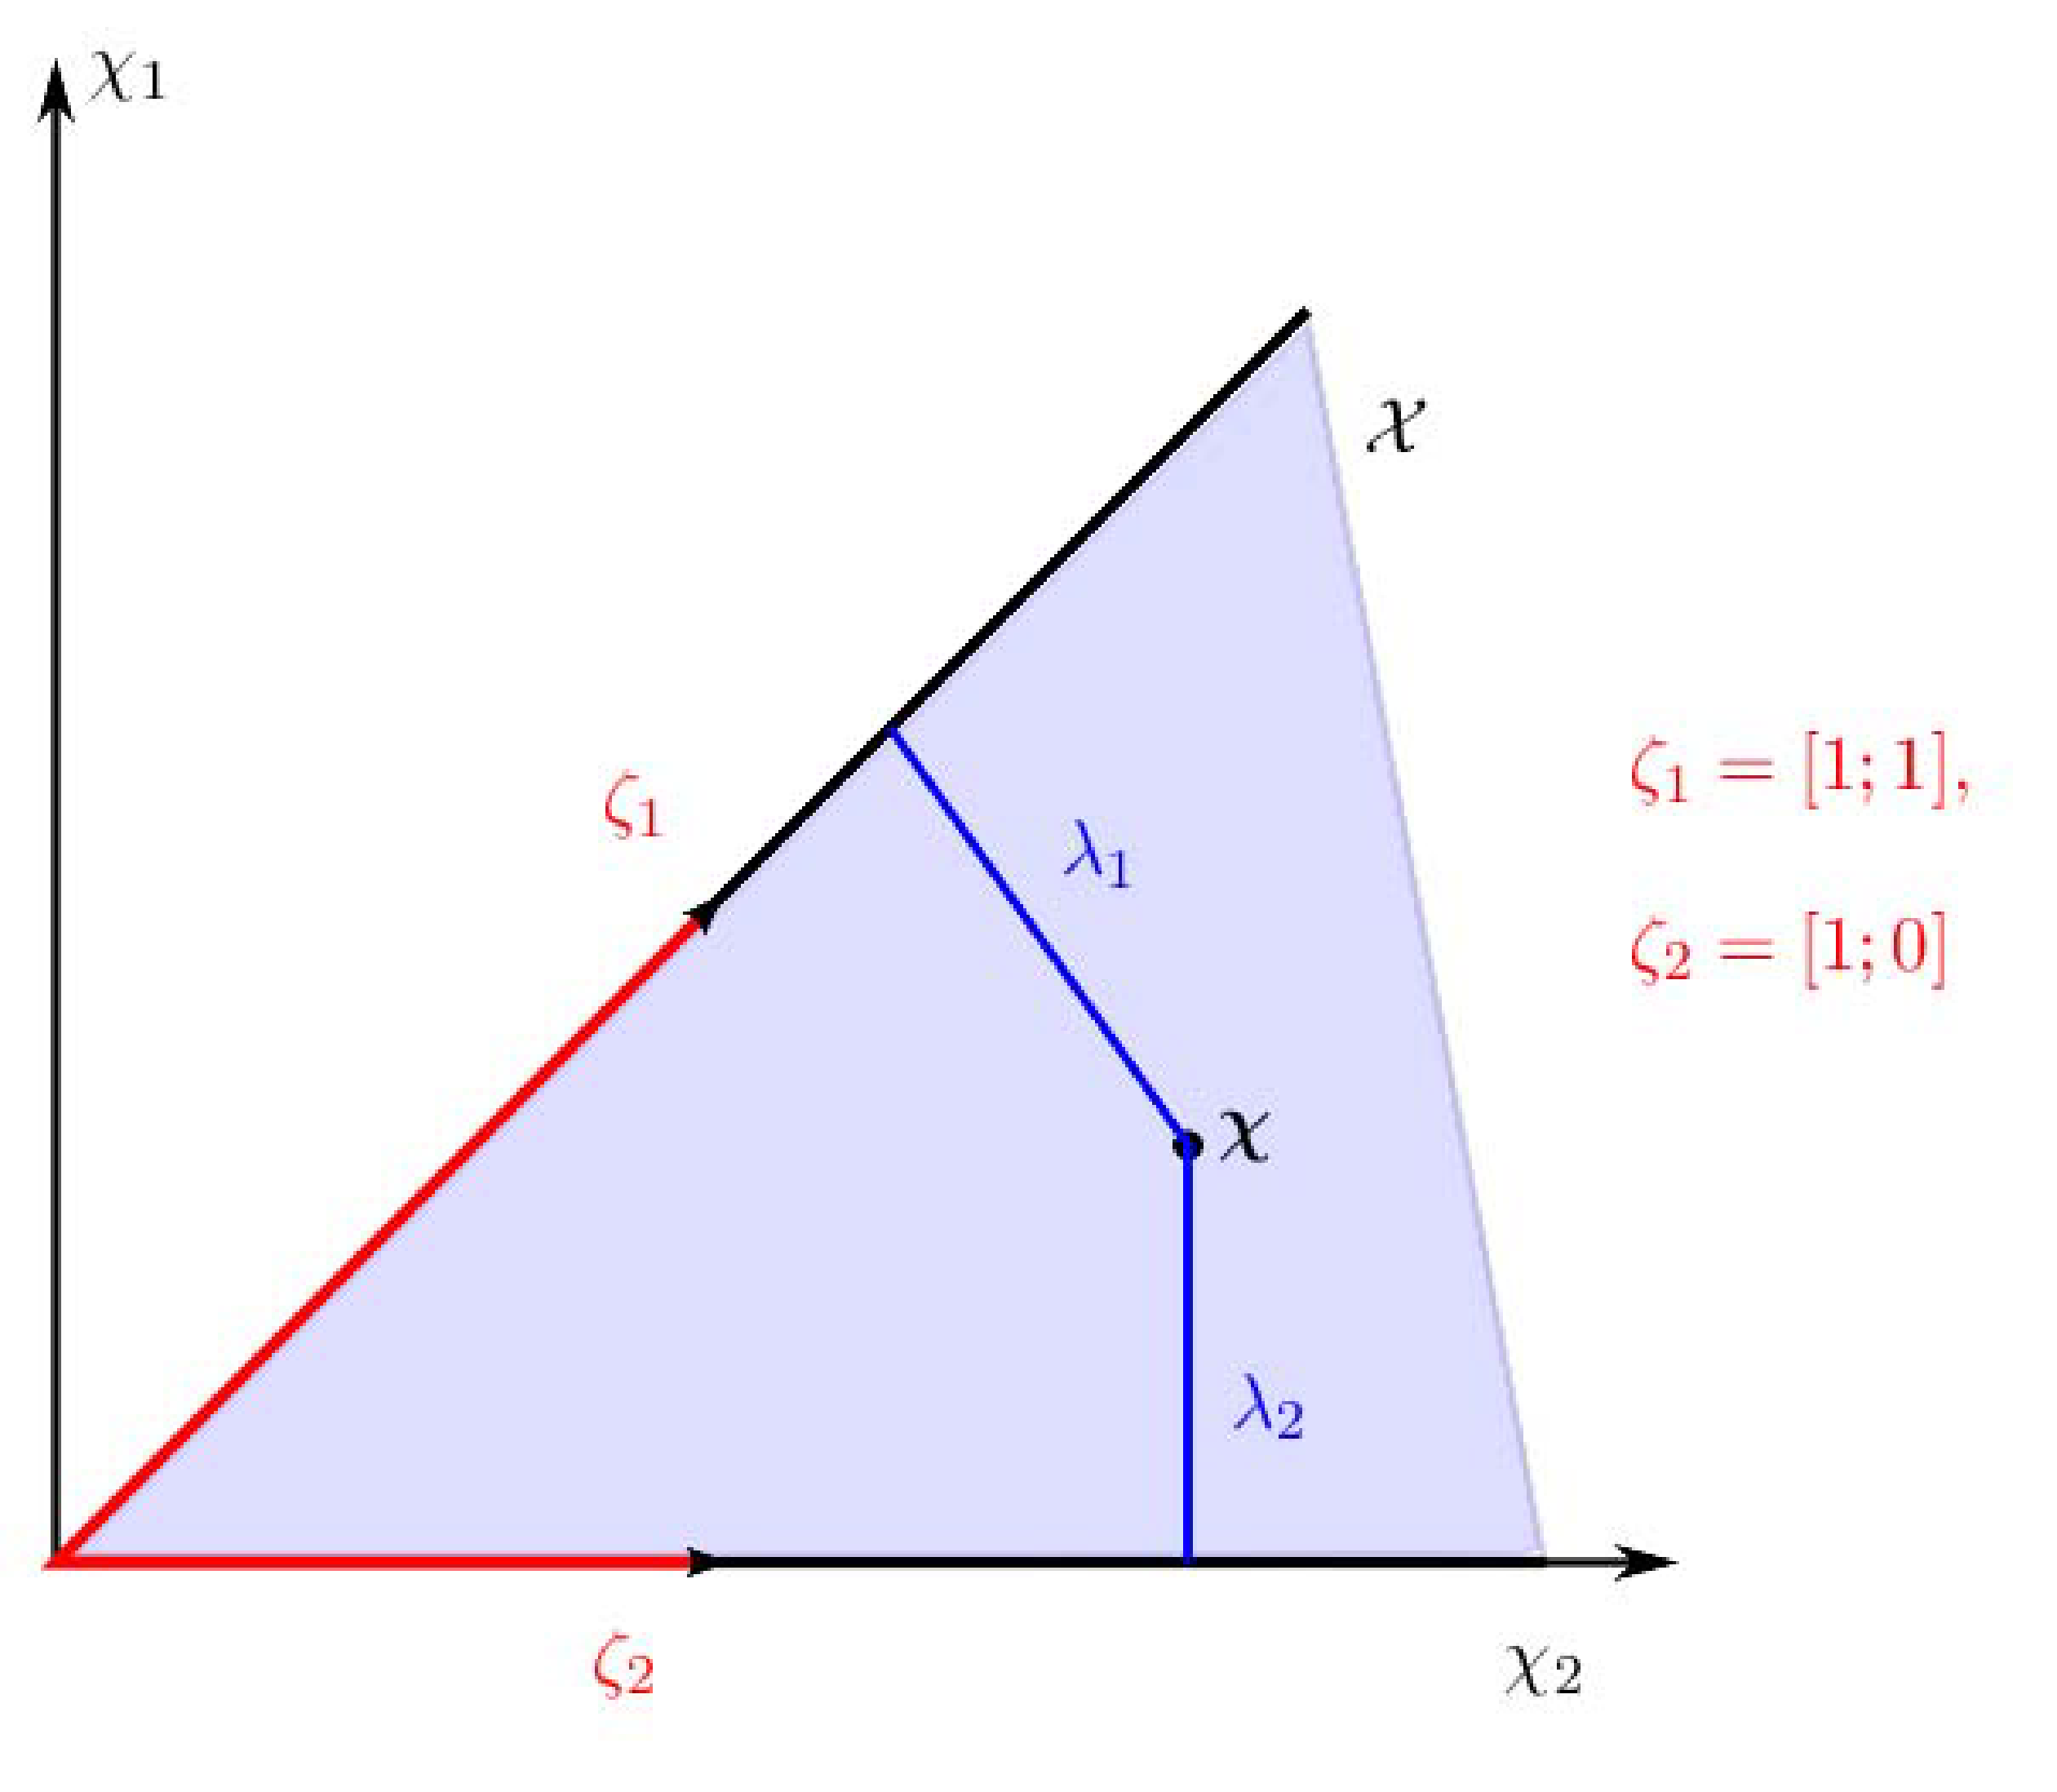
\includegraphics[width=.6\textwidth]{coneTheorem.png}
\caption{Разложение точки по порождающим элементам конуса}
\label{fig:ConeTheorem}
\end{center}
\end{figure}
На рис.~\ref{fig:ConeTheorem} показана иллюстрация теоремы: каждая точка конуса предпочтений, соответствующего множеству из двух элементов~$x_2\succeq x_1$, является неотрицательной комбинацией столбцов матрицы предпочтений~$[1;1]$~и~$[1;0]$ с коэффициентами~$\lambda_1,\lambda_2\geq 0$.


%Помимо конуса~$\cX^A$, рассмотрим полиэдральный конус~$\cX$, представленный неотрицательной комбинацией столбцов матрицы предпочтений~$\bZ$, соответствующей множеству~$X$:
%\begin{equation}
%\cX=\{\bZ\blambda~|~\blambda \geq \mathbf{0}\}.
%\label{eq:ConeGen}
%\end{equation}
%Для конусов~$\cX^A$ и~$\cX$ выполнена следующая теорема.
%\begin{theorem}
%\label{thm:ConeSubset}
%$\cX \subset \cX^A.$
%\end{theorem}

\begin{proof}
Для доказательства утверждения, что конус~$\cX^{\bZ}$ является подмножеством конуса~$\cX$, надо доказать, что справедлива следующая импликация:
\begin{equation}
\blambda\geq 0 \quad \rightarrow \quad \bA\bZ\blambda \leq 0.
\label{eq:ConeSubset}
\end{equation}
Для доказательства этого утверждения достаточно показать, что матрица~$\bA\bZ$ не содержит положительных элементов.

Рассмотрим подробнее элемент~$(\kappa,k)$ матрицы~$\bA\bZ$. Согласно определению матрицы~$\bA$, строка~$\kappa$ матрицы~$\bA$ соответствует паре элементов~$(i,i')$ и содержит два ненулевых элемента, -1 на месте~$i$ и 1 на месте~$i'$, если $x_i\succeq x_{i'}$. При этом соответствующие элементы~$i$ и $i'$ столбца~$k$ матрицы~$\bZ$ могут принимать следующие значения:
\[
(\bZ(i,k),\bZ(i',k))=
\begin{cases}
(1,1),\quad\text{если}\quad x_i\succeq x_k,~x_{i'}\succeq x_k,\\
(0,0),\quad\text{если}\quad x_i\nsucceq x_k,~x_{i'}\nsucceq x_k,\\
(1,0),\quad\text{если}\quad x_i\succeq x_k,~x_{i'}\nsucceq x_k.\\
\end{cases}
\]
Таким образов, элемент $(\kappa,k)$ матрицы~$\bA\bZ$ может принимать лишь два значения:
\[
[\bA\bZ](\kappa,k)=
\begin{cases}
0, \quad\text{если}\quad x_i\succeq x_k,~x_{i'}\succeq x_k \quad \text{или} \quad x_i\nsucceq x_k,~x_{i'}\nsucceq x_k,\\
-1,\quad\text{если}\quad x_i\succeq x_k,~x_{i'}\nsucceq x_k.
\end{cases}
\]
Таким образом, матрица~$\bA\bZ$ не содержит положительных элементов, а, следовательно, справедлива импликация~\eqref{eq:ConeSubset} и включение~$\cX^{\bZ}\subset \cX$.
\end{proof}

Кроме того, для конусов~$\cX$ и~$\cX^{\bZ}$ выполнено следующее утверждение.
\begin{lemm}
\label{lem:ConeEquivLinear}
В случае линейного порядка на множестве~$X$ конусы~$\cX$ и $\cX^{\bZ}$ совпадают.
\end{lemm}
\begin{proof}
Для проведения доказательства перенумеруем элементы линейно упорядоченного множества~$X$ в порядке от большего к меньшему. Построим для отсортированного массива элементов~$x_1,...,x_m\in X$ матрицу~$\bZ$, описывающую отношение порядка между каждой парой объектов. В этом случае, столбец матрицы~$\bZ$ будет состоять из единичного столбца и, возможно, следующего за ним столбца из нулей,~$[1,1,...,1,1,0,0,...,0,0]\T$. Столбец, соответствующий наименьшему объекту из~$X$, будет состоять из единиц.
Допустим, что конусы~$\cX$ и $\cX^{\bZ}$ не совпадают. Это означает, что существует бинарный вектор, являющийся порождающей конуса~$\cX$ и не являющийся столбцом матрицы~$\bZ$. Такой вектор обязательно имеет вид $[...,0_i,1_{i+1}....]$, что нарушает отношение порядка на элементах~$x_i,x_{i+1}$. Таким образом, порождающими конуса~$\cX$ являются только столбцы матрицы~$\bZ$.
\end{proof}

Из доказанной теоремы~\ref{thm:ConeSubset} и леммы~\ref{lem:ConeEquivLinear} следует, что конус предпочтений, представляемый разложением~$\cX^{\bZ}=\{\bZ\blambda~|~\blambda \geq \mathbf{0}\}$, позволяет описывать широкий класс преобразований упорядоченного множества. Разложение конуса~$\cX^{\bZ}$ будет использовано в дальнейших разделах для построения моделей обучения по предпочтениям.


%\section{Решение}
\section{Восстановление предпочтений с использованием конусов}\label{sec:PrefLearnCones}
%Рассматривается задача восстановления отношения предпочтения с использованием порядкового признакового описания.

%\subsection{Восстановление предпочтений с использованием матрицы попарного доминирования объектов}\label{sec:PrefLearnPartMat}
%В этом разделе приведен базовый метод восстановления отношения предпочтения~$z_f$, задаваемого отображением~$f$ на множестве объектов~$X$, $z_f(x_i,x_k)=[f(x_i)\geq f(x_k)]$. Этот метод основывается на восстановлении матрицы предпочтений~$\hat{\bZ}$, каждый элемент которой является линейной комбинацией соответствующих элементов матриц~$\bZ_1,...,\bZ_n$. При этом порядок, определяемый матрицей~$\hat{\bZ}$, оптимально приближает порядок, задаваемый зависимой переменной и соответствующим отношением порядка~$z_0$.

%\paragraph{Мера различия предпочтений.} Для того, чтобы определить понятие оптимальности отношения предпочтения~$z_f$, задаваемого отображением~$f$, введем понятие различия предпочтений~$\rho(z_f,z_0)$. В качестве функции различия будем рассматривать значение отрицательной $\tau$-корреляции между векторами предпочтений, которая, согласно формуле~\eqref{eq:KendZ}, пропорциональна норме Фробениуса между матрицами предпочтений~$\bZ_f$ и $\bZ_0$:
%\begin{equation}
%S(f,X,z_0)=\rho(z_f,z_0)=\|\bZ_f-\bZ_0\|_F\propto -\tau(z_f,z_0).
%\label{eq:ErrFnKend}
%\end{equation}
%Для оптимального восстановления предпочтений требуется найти такое отображение~$f$, матрица~$\bZ_f$ которого минимизирует отклонение~$\rho(z_f,z_0)$. Для решения этой задачи предлагается приближенный алгоритм, описанный в следующем разделе.

%\paragraph{Алгоритм оценивания матрицы предпочтений.} Для нахождения отображения~$f$, минимизирующего~\eqref{eq:ErrFnKend}, предлагается построить матрицу попарного доминирования объектов~$\hat{\bZ}$ с использованием матриц~$\bZ_1,...,\bZ_n$, соответствующих признаковым предпочтениям объектов. Представим каждый элемент матрицы~$\hat{\bZ}$ линейной комбинацией элементов матриц~$\bZ_1,...,\bZ_n$:
%\begin{equation}
%\hat{\bZ}=\sum\limits_{j=1}^n w_j\bZ_j.
%\label{eq:MatEst}
%\end{equation}
%В этом случае, минимизация выражения~\eqref{eq:ErrFnKend} приводит к задаче нахождения оптимальных параметров~$\hat{\bw}$:
%\[
%\hat{\bw} = \arg\min\limits_{\bw}\sum\limits_{i=1}^m\sum\limits_{k=1}^m\left(\bZ_0 - \sum\limits_{j=1}^n w_j\bZ_j\right)^2,
%\]
%где~$\bZ_0$~--- матрица частичного порядка, соответствующая вектору значений зависимой переменной~$\by$. Другими словами, задача построения линейной комбинации матриц является задачей оптимального взвешивания графов предпочтений: матрица~$\hat{\bZ}$ является матрицей инцидентности взвешенного ориентированного графа предпочтений, вес каждого ребра которого определяет степень доминирования между соответствующей парой объектов.


%\begin{eq} Приведем пример линейной комбинации матриц~$\bZ_1,\bZ_2$ согласованных предпочтений. Рассмотрим множество из четырех элементов~$X=\{x_1,x_2,x_3,x_4\}$ и матрицу~$\bZ_1$ из примера~\ref{ex1},
%\[
%\bZ_1=
%\begin{pmatrix}
%1 & 1 & 1 & 1 \\
%0 & 1 & 1 & 1 \\
%0 & 0 & 1 & 0 \\
%0 & 0 & 0 & 1 \\
%\end{pmatrix},
%\]
%соответствующую частичному порядку
%\[
%\begin{diagram}
%\node{x_{1}} \arrow[2]{e}{}
%\node[2]{x_{2}} \arrow[2]{}
%\arrow{se,b}{}
%\node[2]{x_{3}} \\
%\node[4]{x_{4}} %\arrow{ne,r}{C}
%\end{diagram}
%\]
%В качестве матрицы~$\bZ_2$, рассмотрим матрицу
%\[
%\bZ_2=
%\begin{pmatrix}
%1 & 1 & 1 & 1 \\
%0 & 1 & 1 & 1 \\
%0 & 0 & 1 & 1 \\
%0 & 0 & 0 & 1 \\
%\end{pmatrix},
%\]
%соответствующую линейному порядку
%\[
%\begin{diagram}
%\node{x_{1}} \arrow[2]{e}
%\node[2]{x_{2}} \arrow[2]{e}
%\node[2]{x_{3}} \arrow[2]{e}
%\node[2]{x_{4}}
%\end{diagram}
%\]
%Построим матрицу~$\hat{\bZ}$ как линейную комбинацию матриц~$\bZ_1,\bZ_2$ с весами~$w_1=w_2=\frac{1}{2}$:
%\[
%\hat{\bZ}=\frac{1}{2}\bZ_1+\frac{1}{2}\bZ_2=
%\begin{pmatrix}
%1 & 1 & 1 & 1 \\
%0 & 1 & 1 & 1 \\
%0 & 0 & 1 & 1/2 \\
%0 & 0 & 0 & 1 \\
%\end{pmatrix}.
%\]
%Поскольку матрицы~$\bZ_1$ и~$\bZ_2$ соответствуют практически тождественным ранжированиям объектов, только один элемент матрицы~$\hat{\bZ}$ равен~$\frac{1}{2}$, что может быть интерпретировано как неопределенность в доминировании лишь одной пары объектов~$x_3$~и~$x_4$.
%\end{eq}
%
%\begin{eq} Приведем пример линейной комбинации матриц~$\bZ_1,\bZ_2$ несогласованных предпочтений. Рассмотрим матрицу~$\bZ_1$ из предыдущего примера,
%\[
%\bZ_1=
%\begin{pmatrix}
%1 & 1 & 1 & 1 \\
%0 & 1 & 1 & 1 \\
%0 & 0 & 1 & 0 \\
%0 & 0 & 0 & 1 \\
%\end{pmatrix},
%\]
%а в качестве матрицы~$\bZ_2$ рассмотрим матрицу
%\[
%\bZ_2=
%\begin{pmatrix}
%1 & 0 & 0 & 0 \\
%1 & 1 & 0 & 0 \\
%1 & 1 & 1 & 0 \\
%1 & 1 & 1 & 1 \\
%\end{pmatrix},
%\]
%соответствующую линейному порядку
%\[
%\begin{diagram}
%\node{x_{1}}
%\node[2]{x_{2}} \arrow[2]{w}
%\node[2]{x_{3}} \arrow[2]{w}
%\node[2]{x_{4}} \arrow[2]{w}
%\end{diagram}
%\]
%Аналогично предыдущему примеру, построим матрицу~$\hat{\bZ}$ как линейную комбинацию матриц~$\bZ_1,\bZ_2$ с весами~$w_1=w_2=\frac{1}{2}$:
%\[
%\hat{\bZ}=\frac{1}{2}\bZ_1+\frac{1}{2}\bZ_2=
%\begin{pmatrix}
%1 & 1/2 & 1/2 & 1/2 \\
%1/2 & 1 & 1/2 & 1/2 \\
%1/2 & 1/2 & 1 & 0 \\
%1/2 & 1/2 & 1/2 & 1 \\
%\end{pmatrix}.
%\]
%Поскольку матрицы~$\bZ_1$ и~$\bZ_2$ соответствуют противоположным ранжированиям объектов, практически все элементы матрицы~$\hat{\bZ}$ равны~$\frac{1}{2}$, что может быть интерпретировано как неопределенность в попарном доминировании объектов.
%\end{eq}

%\paragraph{Восстановление отношения предпочтения.} Для решения задачи~\eqref{eq:ErrFnKend} необходимо построить матрицу линейного порядка~$\bZ_f$, располагая оценкой матрицы~$\hat{\bZ}$, элементы которой принадлежат отрезку~$[0,1]$. Для того чтобы построить отображение~$f$, воспользуемся идеей из~\cite{Cohen1999}. Будем строить вектор оценок объектов~$\bfx$ в виде суммы столбцов матрицы~$\hat{\bZ}=[\hat{\bz}_1,...,\hat{\bz}_m]$
%\begin{equation}
%\bfx=\sum\limits_{k=1}^m \hat{\bz}_i.
%\label{eq:MatSol}
%\end{equation}
%В работе~\cite{Cohen1999} доказан результат о том, что решение~\eqref{eq:MatSol} в аналогичной постановке является 2-аппроксимацией исходной задачи поиска линейного порядка по матрице доминирования объектов.


Будем строить отображение~$f$ из множества объектов во множество действительных чисел,~$f:X\rightarrow \mathbb{R}$. Для удовлетворения условиям монотонности~\eqref{cond:MonFeat} будем строить множество значений отображения~$f$ в виде суммы конусов предпоятений~$\cX_1,...,\cX_n$~\eqref{df:ConePO}, соответствующим отношениям~$z_1,...,z_n$. Кроме того, определим конус конус целевого предпочтения~$\cY_0$, соответствующий целевому отношению~$z_0$, определенному на~$X$, и будем искать решение задачи в виде ближайших точек конусов.

\subsection{Определение функции потерь с использованием конусного представления предпочтений}\label{subsec:LossFunCone}
%Предложим метод построения оптимизируемой функции потерь для решения задачи восстановления предпочтения~\eqref{prob:PrefLearn}. Для построения функции потерь, определенной на элементах множества~$X$ с заданным на нем отношением частичного порядка~$z_0$, используем представление этого множества в линейном пространстве путем использования конуса~$\cY_0$, соответствующего целевому отношению предпочтения~$z_0$.

Используем понятие конуса частичного порядка~\eqref{df:ConePO} для определения конуса целевого предпочтения.
\begin{df}
Конусом целевого предпочтения~$\cY$ для множества~$X$ с определенным на нем целевым отношением частичного порядка~$z_0$,
\[
z_0=[x_i \succeq_0 x_k],
\]
называется конус, сохраняющий порядок относительно~$z_0$:
\[
\cY=\{\bchi\in\mathbb{R}^m_+|\quad x_i\succeq_0 x_k\rightarrow \chi_{i}\geq \chi_{k}\quad \forall~i,k=1,...,m\}.
\]
\end{df}

%Отметим, что определение~\ref{df:ConeY} является сужением конуса частичного порядка~\eqref{df:ConePO} на элементы выборки~$D$.

Будем строить отображение~$f$ из множества~$X$ во множество действительных чисел~$\mathbb{R}$. Обозначим вектор значений функции~$f$ на множестве~$X$ за~$\bfx\in \mathbb{R}^m$.
\begin{df}
Функцией потерь~$S(f,X,z_0)$ для задачи восстановления предпочтений~\eqref{cond:ErrFnMin} будем называть расстояние от вектора~$\bfx$ до конуса~$\cY$:
\[
S(f,X,z_0)=\min\limits_{\by\in \cY}\|\bfx-\by\|_2,
\]
где~$\|\cdot\|_2$~--- стандартная евклидова норма.
\end{df}
\begin{df}
Решением задачи восстановления предпочтений~\eqref{cond:ErrFnMin} будем называть вектор~$\hat{\bfx}$, минимизирующий значений функции потерь:
\begin{equation}
\hat{\bfx}=\arg\min\limits_{\bfx\in \mathcal{F}}S(f,X,z_0).
\label{prob:ConeOpt}
\end{equation}
\end{df}

%Подробно прямая задача оптимизации~\eqref{prob:ConeOpt} будет рассмотрена в разделе~\ref{sec:ExpEstConc} при согласовании порядковых экспертных оценок.

Отметим, что конус целевого предпочтения~$\cY$, как и любой полиэдральный конус, допускает два представления: полиэдральное и задаваемое конечным набором порождающих элементов. Порождающее представление определяется конусом~$\cY^{\bZ_0}$, который является подмножеством конуса~$\cY$, и задается неотрицательной линейной комбинацией столбцов матрицы~$\bZ_0$:
\begin{equation}
\cY\supset\cY^{\bZ_0}=\{\bZ_0\blambda_0~|~\blambda_0\geq\mathbf{0}\},
\label{eq:FinGenY}
\end{equation}
где~$\bZ_0$~--- матрица предпочтений, соответствующая целевому отношению предпочтения~$z_0$, определенному на~$X$.

В этом случае, функция потерь~$S(f,X,z_0)$ записывается следующим образом:
\begin{equation}
S(f,X,z_0)=\min\limits_{\blambda_0 \geq 0}\|\bfx-\bZ_0\blambda_0\|_2.
\label{eq:LossFinGen}
\end{equation}

%Функция потерь~\eqref{eq:LossFinGen} является справедливой в случае, когда на множестве меток~$Y$ задано отношение нестрогого частичного порядка. В случае, когда на~$Y$ задано отношение строгого порядка (например, в задаче порядковой классификации,~$Y=\{y_1\succ...\succ y_K\}$), необходимо рассматривать лишь внутренние точки конуса~$\cY$, то есть все элементы вектора~$\blambda_0$ должны быть положительными,~$\blambda_0 > \mathbf{0}$. Выполнение этого условия можно достигнуть введением дополнительного ограничения в задачу~\eqref{eq:LossFinGen}, например
%\[
%S(f,X,z_0)=\min\limits_{\blambda_0 \geq \tau \mathbf{1},~\tau > 0}\|\bfx-\bZ_0\blambda_0\|_2.
%\]
В данной работе мы будем рассматривать упрощенный подход на основе использования центральной точки конуса~$\cY$, то есть случай~$\blambda_0=\mathbf{1}$, и оптимизировать функцию потерь
\begin{equation}
S(f,X,z_0)=\|\bfx-\bZ_0\mathbf{1}\|_2.
\label{eq:LossFinGenStrict}
\end{equation}

%\paragraph{Полиэдральное представление конуса~$\cY_0$.} Помимо порождающего представления~\eqref{eq:FinGenY}, согласно определению~\ref{df:Cone}, конус целевого предпочтения~$\cY_0$ допускает также полиэдральное представление следующего вида:
%\begin{equation}
%\cY_0=\{\by~|~\bA\by\leq 0\},
%\label{eq:PolyhedY}
%\end{equation}
%где матрица~$\bA$ имеет размеры~$m^2\times m$ и описывает отношение предпочтения между каждой парой объектов: в строке матрицы~$\bA$, соответствующей паре объектов~$i,k$ содержится не более двух ненулевых элементов:~$-1$ на $i$-м месте и 1 на $k$-м месте, если для объектов~$i,k$ выполняется~$x_i\succeq_0 x_k$.
%
%Цель оптимизационной задачи~\eqref{prob:ConeOpt} заключается в том, чтобы найти вектор~$\bfx$, принадлежащий конусу~$\cY_0$. Согласно полиэдральному представлению~\eqref{eq:PolyhedY}, вектор~$\bfx$ должен выполнять условие
%\[
%\bA\bfx\leq \mathbf{0}.
%%\label{cond:MonA}
%\]
%При этом в случае строгого отношения порядка, определенного на элементах множества~$Y$, рассматривается строгий вариант неравенства~\eqref{eq:PolyhedY},
%\begin{equation}
%\bA\bfx< \mathbf{0}.
%\label{cond:MonA}
%\end{equation}
%Отметим, что векторное неравенство~\eqref{cond:MonA} эквивалентно предъявляемым условиям монотонности~\eqref{cond:Mon}. Условие~\eqref{cond:MonA} переформулировывается в виде задачи минимизации количества положительных элементов вектора~$\bA\bfx$, что приводит к стандартной оптимизационной задаче:
%\begin{equation}
%S(f,X,z_0)=\sum\limits_{x_i\succ_0 x_k}[f(x_i)\leq f(x_k)].
%\label{eq:LossPolyhed}
%\end{equation}
%
%В работе~\cite{liu2007supervised} для выполнения условия~\eqref{cond:MonA} рассматривается оптимизационная задача с использованием дополнительного вектора переменных $\mathbf{t}$:
%\[
%\min\limits_{\mathbf{t}\geq\mathbf{0}} \|\mathbf{t}\|_2,\quad \bA\bfx < \mathbf{t}.
%\]
%
%Кроме того, при использовании кусочно-линейной аппроксимации функции потерь и введении регуляризатора на вектор параметров модели, задача~\eqref{eq:LossPolyhed} переписывается в терминах стандартного функционала RankSVM~\eqref{eq:LossRankSVM}.
%
%Путем использования полиэдрального~\eqref{df:Cone} и порождающего~\eqref{df:ConeGen} представлений конуса целевого предпочтения~$\cY_0$ сформулировано две оптимизационные задачи.  Первая задача~\eqref{eq:LossFinGen} заключается в минимизации расстояния до конуса~$\cY$. Вторая задача~\eqref{eq:LossPolyhed} минимизирует количество невыполняемых ограничений-неравенств. Отметим, что стандартные функции потерь, рассматриваемые в задачах попарного ранжирования~\cite{cao2006adapting, Trotman2005} являются аппроксимацией выражения~\eqref{eq:LossPolyhed} и соответствуют \emph{попарному подходу} к задаче ранжирования. В свою очередь, задача поиска ближайших точек в конусах~\eqref{eq:LossFinGen} соответствует и обобщает \emph{поточечный подход} к задаче: параметры неотрицательной комбинации~$\blambda_0$ в конусе~$\cY$ играют роль разделителей числовой оси на конечное множество меток. В последующих разделах в основном будет использоваться вариант~\eqref{eq:LossFinGenStrict}.

\subsection{Линейная полиэдральная модель восстановления предпочтений}\label{subsec:LinPolyhedMdl}
В этом подразделе определим линейную полиэдральную модель для решения задачи восстановления предпочтения. Модель основывается на построении суммы конусов предпочтений, соответствующих порядковым признакам.

Как и ранее, множество объектов~$X=\{x_1,...,x_m\}$ задано порядковым описанием: на~$X$ задано~$n$ отношений частичного порядка~$z_1,...,z_n$. Каждому из отношений~$z_j$ соответствует конус предпочтений~$\cX_j\subset \mathbb{R}^m$, определяемый формулой~\eqref{df:ConePO}, а также конус~$\cX^{\bZ_j}\subset \cX_j$, порождаемый столбцами матрицы предпочтений~$\bZ_j$.

 Напомним определение \emph{суммы Минковского} двух множеств.
\begin{df}
Суммой Минковского двух подмножеств~$\cX_1,\cX_2$ линейного пространства является множество, состоящее из сумм всевозможных векторов из~$\cX_1$~и~$\cX_2$:
\[
\cX_1\oplus \cX_2 =\{\bchi~|~\bchi=\bchi_1+\bchi_2,~\bchi_1\in \cX_1,~\bchi_2\in \cX_2\}.
\]
\end{df}

Будем строить множество значений отображения~$f$ в виде суммы Минковского конусов~$\cX^{\bZ_1},...,\cX^{\bZ_n}$. Для этого определим множество значений линейной полиэдральной модели.
\begin{df}
Множеством значений линейной полиэдральной модели~$f$ на объектах, $\bfx(x_1,...,x_m)$, назовем сумму Минковского конусов $\cX^{\bZ_1},...,\cX^{\bZ_n}$:
\begin{equation}
\bfx(x_1,...,x_m)~\in~\cX^{\bZ_1}\oplus ... \oplus \cX^{\bZ_n}~\subset~\mathbb{R}^m.
\label{df:LinPolyhedSet}
\end{equation}
\end{df}

Каждый вектор конуса~$\cX^{\bZ_j}$ представим в виде неотрицательной комбинации столбцов матрицы частичного порядка~$\bZ_j$. Используя этот факт, множество значений линейной полиэдральной модели на объектах $x_1,...,x_m$ представляется следующим образом.
\begin{lemm}
Значением линейной полиэдральной модели~$f$ на объектах~$x_1,...,x_m$ является неотрицательная линейная комбинация вида
\begin{equation}
\bfx(x_1,...,x_m)~=~\sum\limits_{j=1}^n\bZ_j\blambda_j,~\blambda_j\geq 0.
\label{lem:LinPolyhedMdl}
\end{equation}
\end{lemm}
Доказательство этой леммы следует непосредственно из формулы~\eqref{eq:ConeGen} и определения~\eqref{df:LinPolyhedSet}.
Важным следствием разложения~\eqref{lem:LinPolyhedMdl} является возможность определения линейной полиэдральной модели на произвольном объекте~$x\in \mathbb{X}$.
\begin{df}
Линейной полиэдральной моделью~$f:\mathbb{X}\rightarrow\mathbb{R}$ является отображение вида
\begin{equation}
f(x)~=~\sum\limits_{j=1}^n\bz_j\T\blambda_j,~\blambda_j\geq \mathbf{0},
\label{df:LinPolyhedMdl}
\end{equation}
где~$\bz_j$~--- вектор индикаторов доминирования объектом~$x$ объектов~$x_1,...,x_m$ согласно отношению предпочтения~$z_j$:
\[
\bz_{j}(k)=[x\succeq_j x_k],
\]
где~$\bz_j(k)$~--- $k$-й элемент вектора~$\bz_j$.
\end{df}

%Следующие подразделы посвящены оценкам параметров модели~\eqref{df:LinPolyhedMdl} с использованием целевого отношения предпочтения~$z_0$ и соответствующего ему конуса частичного порядка~$\cY_0$. В подразделе~\ref{subsec:ParEstDirect} рассматривается прямой метод оценки параметров на основе решения задачи неотрицательной линейной регрессии. В подразделе~\ref{subsec:ConeReg} рассматривается метод регуляризации модели с использованием центральных точек конусов. Наконец, в подразделе~\ref{subsec:ParEstPolyhed} рассматривается метод построения суммы Минковского~\eqref{df:LinPolyhedSet} с использованием полиэдрального представления конусов частичного порядка.

\subsubsection{Прямая оценка параметров полиэдральной модели}
\label{subsec:ParEstDirect}

Рассматривается задача минимизации функции потерь~$S(f,X,z_0)$ вида~\eqref{eq:LossFinGenStrict}, где~$f$ является линейной полиэдральной моделью вида~\eqref{lem:LinPolyhedMdl}:
\[
\bfx(x_1,...,x_m)~=~\sum\limits_{j=1}^n\bZ_j\blambda_j,~\blambda_j\geq 0,
\]
для определения оптимальных параметров~$\blambda_j$.

В данном разделе предлагается прямая оценка параметров модели~\eqref{lem:LinPolyhedMdl}, построенной на основе суммы Минковского конусов предпочтений. Для решения оптимизационной задачи разработан алгоритм оценки параметров модели.

Оптимальные параметры~$\blambda_1,...,\blambda_n$ должны минимизировать функцию потерь~\eqref{eq:LossFinGenStrict}.
С учетом явного вида модели~$\bfx$ задача поиска оптимальных параметров записывается следующим образом:
\begin{equation}
(\hat{\blambda}_1,...,\hat{\blambda}_n)=\mathop{\arg\min}\limits_{\blambda_1,...,\blambda_n\geq \mathbf{0}}\|\bZ_0\mathbf{1}-\sum\limits_{j=1}^n\bZ_j\blambda_j\|_2.
\label{eq:LossConicDirect}
\end{equation}

Задача~\eqref{eq:LossConicDirect} является задачей \emph{неотрицательной линейной регрессии} с матрицей~$[\bZ_1,\bZ_2,...,\bZ_n]$, являющейся присоединением всех матриц~$\bZ_1,...,\bZ_n$, соответствующих порядковым признакам. Для решения этой задачи в~\cite{lawson1974solving, chen2009nonnegativity} предложен подход на основе \emph{метода активного множества}. В данной работе предлагается использовать этот метод для итеративного решения задачи неотрицательной линейной регрессии последовательно для всех матриц~$\bZ_1,...,\bZ_n$.
\sloppy{}

Обозначим за~$\hat{\blambda}^t_j$ оценку~$j$-го вектора параметров, полученную на шаге~$t$. Алгоритм итеративной оценки параметров заключается в следующем.
\begin{enumerate}
\item На начальном шаге присвоить всем элементам вектора параметров равные значения~$\hat{\lambda}^0_{jk}=1/m$. В этом случае каждый вектор~$\hat{\blambda}^0_j$ является центральной точкой конуса~$\cX_j$.
\item На шаге~$t$ провести последовательную оценку параметров~$\hat{\blambda}^t_j$ для всех~$j=1,...,n$. Для этого предполагаются фиксированными все векторы~$\hat{\blambda}^t_1,...,\hat{\blambda}^t_{j-1},\hat{\blambda}^{t-1}_{j+1},...,\hat{\blambda}^{t-1}_{n}$, и вектор~$\hat{\blambda}^t_j$ отыскивается путем минимизации функции потерь:
\begin{equation}
\hat{\blambda}^t_j=\arg\min\limits_{\blambda_j\geq\mathbf{0}}\|\bZ_0\mathbf{1}-\sum\limits_{j'=1}^{j-1}\bZ_{j'}\hat{\blambda}^t_{j'}-\sum\limits_{j'=j+1}^{m}\bZ_{j'}\hat{\blambda}^{t-1}_{j'}-\bZ_j\blambda_j\|_2.
\label{eq:LinearPolyhedEstimStep}
\end{equation}
Каждая из задач~\eqref{eq:LinearPolyhedEstimStep} является задачей неотрицательной линейной регрессии и решается методом активного множества.
\end{enumerate}

\subsubsection{Оценка параметров с использованием центральной точки конуса}
\label{subsec:ConeReg}
В данном подразделе рассматривается задачи минимизации функции потерь~\eqref{eq:LossConicDirect} на сокращенном пространстве параметров.
Для сокращения размерности пространства параметров используем понятие центральной точки полиэдрального конуса. %Показано, что использование центральных точек приводит к задаче максимизации~$\tau$-корреляции~\eqref{eq:ErrFnKend}.
\begin{df}
Центральной точкой полиэдрального конуса~$\cX$, задаваемого конечным набором порождающих элементов~$\bzeta_{k}$,
\[
\cX=\{\bchi~|~\bchi=\sum\limits_{k=1}^{r}\lambda_{k}\bzeta_{k},~\lambda_{k}\geq 0\},
\]
является точка~$\overline{\bx}$ вида
\[
\overline{\bx}=\frac{1}{r}\sum\limits_{k=1}^{r}\bzeta_{k}.
\]
\end{df}
\begin{figure}[h]
\begin{center}
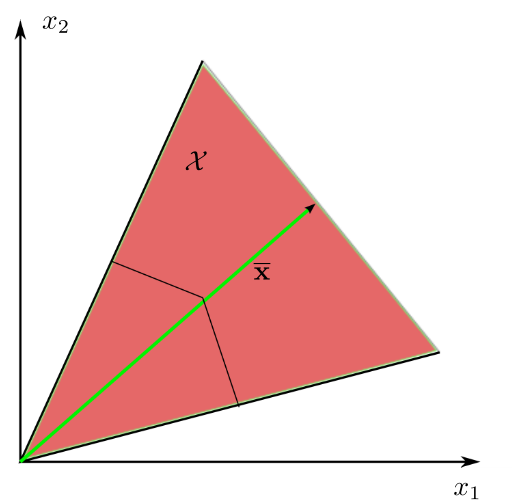
\includegraphics[width=.5\textwidth]{coneCentralPoint.png}
\caption{Центральная точка конуса}
\label{fig:ConeCentralPoint}
\end{center}
\end{figure}
Другими словами, центральной точкой конуса является центральная точка выпуклой комбинации его порождающих элементов. Изображение центральной точки показано на рис.~\ref{fig:ConeCentralPoint}.

Перепишем формулу~\eqref{lem:LinPolyhedMdl} следующим образом:
\[
\bfx(x_1,...,x_m)~=~\sum\limits_{j=1}^n\bZ_j\blambda_j=\sum\limits_{k=1}^m\sum\limits_{j=1}^n\bz_{jk}\lambda_{jk},
\]
где~$\bz_{jk}$~--- столбец~$k$ матрицы~$\bZ_j$. Выделив в этой комбинации переменные~$w_j=\sum\limits_{k=1}^n \lambda_{jk}$, получим
\[
\bfx(x_1,...,x_m)~=\sum\limits_{k=1}^m\sum\limits_{j=1}^n w_j \bz_{jk}\lambda'_{jk},
\]
где~$\lambda'_{jk}=\frac{\lambda_{jk}}{w_j}$ для всех ненулевых~$w_j$. При этом выполняются условия нормированности параметров~$\lambda'_{jk}$, а также неотрицательности всех параметров:
\[
\sum\limits_{j=1}^n\lambda'_{jk}=1,~\blambda'_j\geq\mathbf{0},~w_j\geq 0.
 \]
Для дальнейшего удобства переобозначим параметры~$\lambda_{jk}:=\lambda'_{jk}$.

Рассмотрим конус~$\cX_k^w$, порождаемый элементами $w_j \bz_{jk}$. Для снижения размерности пространства параметров, заменим в модели~$f$ конус~$\cX_k^w$ его центральной точкой. В этом случае для модели~$\bfx$ получим следующее выражение:
\[
\bfx(\bx_1,...,\bx_m)~=\sum\limits_{k=1}^m \lambda_k \bz^w_{jk},
\]
где
\[
\bz^w_{jk}=\sum\limits_{j=1}^n w_j \bz_{jk},\quad\sum\limits_{k=1}^m\lambda_k=1.
\]

Таким образом, доказана следующая теорема о регуляризации линейной полиэдральной модели с помощью центральных точек конусов.
\begin{theorem}
При замене конуса~$\cX_k^w$ его центральной точкой~$\overline{\bx}_k^w=\frac{1}{n}\sum\limits_{j=1}^{n}w_j \bz_{jk}$ линейная полиэдральная модель~\eqref{lem:LinPolyhedMdl} принимает следующий вид:
\begin{equation}
\bfx(\bx_1,...,\bx_m)=\hat{\bZ}\blambda,\quad \hat{\bZ}=\sum\limits_{j=1}^nw_j\bZ_j,
\label{eq:LinRegMdl}
\end{equation}
при ограничениях
\[
w_j\geq 0,~\sum\limits_{k=1}^m\lambda_k=1,~\blambda\geq\mathbf{0}.
\]
\end{theorem}

Матрица~$\hat{\bZ}$ описывает отношение частичного порядка между каждой парой объектов выборки. Элемент этой матрицы~$\hat{\bZ}(i, k)$ может быть интерпретируем как степень достоверности того, что объект~$x_i$ доминирует объект~$x_k$,~$x_i\succeq x_k$.

\paragraph{Минимизация функции потерь для поиска оптимальных параметров} Оптимизационная задача~\eqref{eq:LossConicDirect} с учетом регуляризации~\eqref{eq:LinRegMdl} представляется следующим образом:
\begin{equation}
(\hat{\bw},\hat{\blambda})=\arg\min\limits_{\bw,\blambda}\|\bZ_0\mathbf{1}-\left(\sum\limits_{j=1}^nw_j\bZ_j\right)\blambda\|_2,
\label{eq:LossConicReg}
\end{equation}
\[
w_j\geq 0,~\sum\limits_{k=1}^m\lambda_k=1,~\blambda\geq\mathbf{0}.
\]

Справедлива следующая лемма о том, функция потерь~\eqref{eq:LossConicReg} ограничена сверху нормой разности матриц $\|\bZ_0-\hat{\bZ}\|_F$, являющейся отрицательной~$\tau$-корреляцией отношений~$z_0$ и $z_f$.
\begin{lemm}
$\min\limits_{\blambda\geq\mathbf{0},~\|\blambda\|_1=1}\|\bZ_0\mathbf{1}-m\hat{\bZ}\blambda\|_2\leq \|\bZ_0-\hat{\bZ}\|_F$.
\end{lemm}
\begin{proof}
\[
\min\limits_{\blambda\geq\mathbf{0},~\|\blambda\|_1=1}\|\bZ_0\mathbf{1}-m\hat{\bZ}\blambda\|_2=\min\limits_{\blambda\geq\mathbf{0},~\|\blambda\|_1=m}\|\bZ_0\mathbf{1}-\hat{\bZ}\blambda\|_2\leq\|\bZ_0\mathbf{1}-\hat{\bZ}\mathbf{1}\|_2\leq \|\bZ_0-\hat{\bZ}\|_F.
\]
\end{proof}

Доказанное утверждение позволяет свести задачу~\eqref{eq:LossConicReg} к задаче восстановления отношения предпочтения на основе минимизации нормы разности матриц~$\bZ_0$ и~$\bZ_f$.

Оценку параметров модели~\eqref{eq:LossConicReg} проведем в два этапа. На первом этапе оценим матрицу частичного порядка~$\hat{\bZ}$, являющуюся линейной комбинацией матриц~$\bZ_1,...,\bZ_n$,
\begin{equation}
\hat{\bZ}=\sum\limits_{j=1}^n w_j\bZ_j,
\label{eq:MatEst}
\end{equation}
путем минимизации функции ошибки
\begin{equation}
\hat{\bw} = \arg\min\limits_{\bw}\sum\limits_{i=1}^m\sum\limits_{k=1}^m\left(\bZ_0 - \sum\limits_{j=1}^n w_j\bZ_j\right)^2.
\label{eq:MatSol}
\end{equation}
На втором этапе оценим параметры~$\blambda$ линейной комбинации $\hat{\bZ}\blambda$ методом неотрицательной линейной регрессии.


\paragraph{Пример: задача порядковой классификации.} Используем оценку~\eqref{eq:MatEst} матрицы~$\hat{\bZ}$ для задачи многоклассовой порядковой классификации, являющейся частным случаем задачи восстановления предпочтения с конечным множеством меток~$Y=\{l_1,l_2,...,l_K\}$ с заданным на нем отношением строгого линейного порядка,~$l_1\prec l_2,...,\prec l_K$. Требуется построить монотонное отображение~$f:X\rightarrow Y$, доставляющее минимум функции ошибки порядковой классификации. Располагая оценкой матрицы частичного порядка~$\hat{\bZ}$, оценим параметры~$\lambda_k$ в линейной комбинации $\bfx = \hat{\bZ}\blambda$.

Воспользуемся методом порядковой логистической регрессии для оценки параметров~$\lambda_k$. Классифицируем объект~$x_i$ следующим образом:
\[
\hat{y}_i=
\begin{cases}
y_1,~\text{если}~f(x_i) \leq \mu_1, \\
y_2,~\text{если}~\mu_1 < f(x_i) \leq \mu_2, \\
..., \\
y_K,~\text{если}~\mu_K < f(x_i),
\end{cases}
\]
где~$f(x_i)$ является оценкой объекта~$x_i$, компонентой~$i$ вектора оценок~$\bfx$, построенного по правилу~$\bfx=\hat{\bZ}\blambda$.

Здесь $\mu_1,...,\mu_K$ являются параметрами решающего правила, разделяющими числовую ось~$\mathbb{R}$ на области принадлежности меткам классов~$y_k$. Оптимальные параметры подбираются путем минимизации функции потерь~$S$,
\[
S(\blambda, \boldsymbol{\mu})=-\sum\limits_{i=1}^m \log\left(\sigma(\mu_{y_i}-\blambda\T \hat{\bz}_i) - \sigma(\mu_{y_{i-1}} - \blambda\T \hat{\bz}_i)\right)\rightarrow \min,
\]
где~$\sigma$~--- сигмоидная функция,
\[
\sigma(t)=1/\bigl(1 + \exp{(-t)}\bigr),
\]
а~$\bz_i$~--- вектор-столбец~$i$ матрицы~$\hat{\bZ}$.

%Применение данного подхода будет продемонстрировано в экспериментальной части работы в разделе решения задачи порядковой классификации на данных UCI. Результаты классификации превосходят результаты многих известных алгоритмов.

\section{Эксперимент}
Этот раздел посвящен анализу и иллюстрации предложенных методов на прикладных задачах. Рассматривается задача категоризации Красной книги РФ~\cite{stenina2015ordinal} и задача порядковой классификации на наборах данных из репозитория UCI~\cite{asuncion2007uci}.

В Красной книге Российской Федерации приняты следующие категории статуса редкости таксонов (видов, подвидов, популяций) животных:
\begin{enumerate}
\setcounter{enumi}{-1}
\item Вероятно исчезнувшие.
\item Находящиеся под угрозой исчезновения.
\item Сокращающиеся в численности.
\item Редкие.
\item Неопределенные по статусу.
\item Восстанавливаемые и восстанавливающиеся.
\end{enumerate}

\begin{table}
\caption{Экспертное признаковое описание объектов Красной книги РФ}
\label{Table:IUCN}
\begin{center}
\begin{tabular}{|r|c|c|c|c|c|c|c|c|c|}
\hline
\begin{sideways}Названия таксонов\end{sideways} & \begin{sideways}Азовская белуга\end{sideways} &\begin{sideways}Сибирский осетр\end{sideways}
&\begin{sideways}Сахалинский осетр\end{sideways} &\begin{sideways}Волховский сиг\end{sideways}
&\begin{sideways}Длинноперая палия\end{sideways} &\begin{sideways}Кильдинская треска\end{sideways}
&\begin{sideways}Белый медведь\end{sideways} &\begin{sideways}Желтозобик\end{sideways} &\begin{sideways}Кулик-лопатень\end{sideways}\\
\hline
Численность & 1 & 2 & 2 & 2 & 3 & 2 & 3 & 2 & 2 \\
\hline
Плотность & 1 & 2 & 1 & 2 & 3 & 2 & 3 & 2 & 2 \\
\hline
Площадь ареала & 3 & 2 & 2 & 2 & 1 & 1 & 3 & 1 & 1 \\
\hline
Структура ареала & 5 & 5 & 4 & 5 & 5 & 5 & 5 & 2 & 2 \\
\hline
Структура популяции & 1 & 2 & 0 & 2 & 0 & 1 & 1 & 1 & 1 \\
\hline
Генетическое разнообразие & 1 & 0 & 0 & 1 & 0 & 1 & 0 & 0 & 0 \\
\hline
Физиологическое состояние & 2 & 3 & 3 & 3 & 3 & 3 & 3 & 3 & 2 \\
\hline
Изменение размера популяции & 1 & 2 & 2 & 3 & 3 & 0 & 4 & 3 & 2 \\
\hline
\textbf{Экспертная категоризация} & \textbf{1} & \textbf{2} & \textbf{1} & \textbf{2} & \textbf{3} & \textbf{1} & \textbf{5} & \textbf{3} & \textbf{3} \\
\hline
\end{tabular}
\end{center}
\end{table}


Каждый таксон описан набором признаков, отражающих его состояние. Предполагается, что текущая версия Красной книги РФ составлена <<в~целом>> непротиворечиво, то есть, существует соответствие между описанием вида и его статусом. Эксперт, владеющий информацией о таксоне, выставляет порядковую оценку для каждого признака. Таким образом, задана матрица <<объект-признак>>~(табл.~\ref{Table:IUCN}), состоящая из описаний таксонов, и вектор меток классов таксонов.
Требуется построить отображение, восстанавливающую класс таксона из Красной книги РФ по его описанию. Это отображение должно принимать значения на линейно упорядоченном множестве статусов таксона.

%Задача ревизии Красной книги РФ и построения модели оценок таксонов является актуальной из-за постоянного пополнения книги новыми записями о таксонах.
%
%Используются следующие предположения о составе и свойствах признаков:
%\begin{enumerate}
%    \item[1)] оцениваемый экспертами состав признаков считается исчерпывающим для получения модели;
%    \item[2)] учитывается структура на признаках;
%    \item[3)] на значениях признаков задано отношение полного порядка, кроме пропущенного значения;
%    \item[4)] выполняется правило <<the bigger the better>>, то есть большему (благоприятному) значению признака соответствует больший (благоприятный) статус вида;
%    \item[5)] различные экспертные оценки по одному и тому же виду приветствуются;
%    \item[6)] каждый из признаков принимает на выборке все допустимые значения и только их, при нарушении условия ставится вопрос о корректности анкеты;
%    \item[7)] признак отвергается, если более половины значений пропущены.
%\end{enumerate}

Для решения этой задачи были использованы следующие подходы: подходы на основе оценивания матрицы предпочтений, подход на основе конусов, метод криволинейной регрессии и подход на основе копул (все подходы описаны в главе~\ref{ch:PrefLearn}), а также метод решающих деревьев (Trees), порядковый метод опорных векторов (SVM)~\cite{frank2001simple} и метод классификации на основе ближайших соседей с монотонными ограничениями (KNN), описанный в~\cite{duivesteijn2008knn}.

Эксперимент проводился на выборке, состоящей из экспертных оценок видов Красной книги РФ и экспертных оценок важности признаков. В выборку вошли 102 объекта из трех категорий риска, описанные 102-мя признаками (равенство числа объектов и признаков является случайным совпадением). Признаки представлены в таблице на рис.~\ref{fig:criterion_table}.

Для оценки качества алгоритмов в этом подразделе рассматривается средняя потеря Хэмминга~$L_H(\by,\hat{\by})$, задаваемая формулой
\begin{equation}
L_H(\by,\hat{\by})=\frac{1}{m}\sum\limits_{i=1}^m|y_i-\hat{y_i}|_H,
\label{eq:LossHamming}
\end{equation}
где~$\by$~-- заданная целевая переменная, а~$\hat{\by}$~--- его оценка. Отметим, что множество значений вектора~$\by$ является упорядоченным множеством меток~$Y=\{y_1\succ...\succ y_k\}$, поэтому в качестве нормы~$\|\cdot\|_H$ рассматривается функция Хэмминга~\cite{stenina2015ordinal}.
Ниже представлены графики сходимости методов и результаты их сравнения.

\paragraph{Алгоритм прямой оценки параметров полиэдральной модели.}
\begin{figure}
\begin{center}
\subfloat[Сходимость параметров]{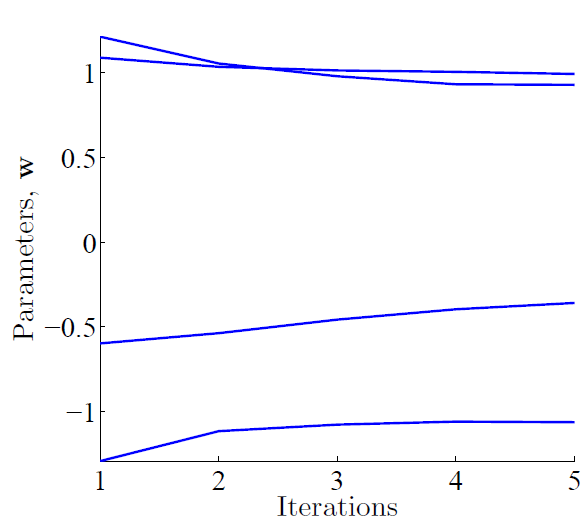
\includegraphics[width=.4\textwidth]{ConesConvPar1.png}\label{subfig:ConesConvPar1}}
\subfloat[Значение ошибки]{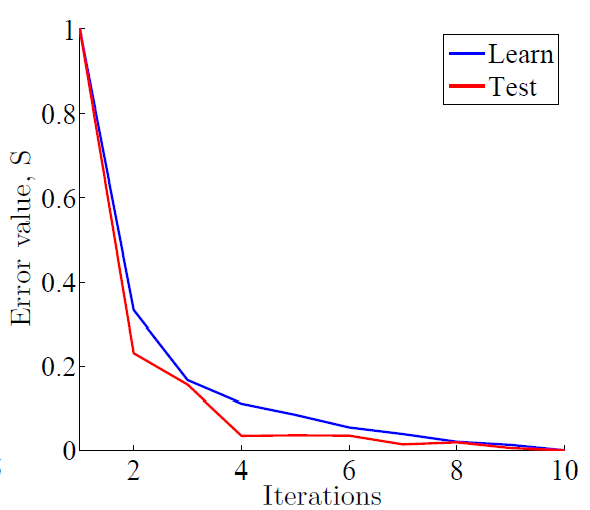
\includegraphics[width=.4\textwidth]{ConesConvErr1.png}\label{subfig:ConesConvErr1}} \\
\caption{Сходимость параметров полиэдральной модели, случай малого количества параметров}
\label{fig:ConesConvSmall}
\end{center}
\end{figure}

\begin{figure}
\begin{center}
\subfloat[Сходимость параметров]{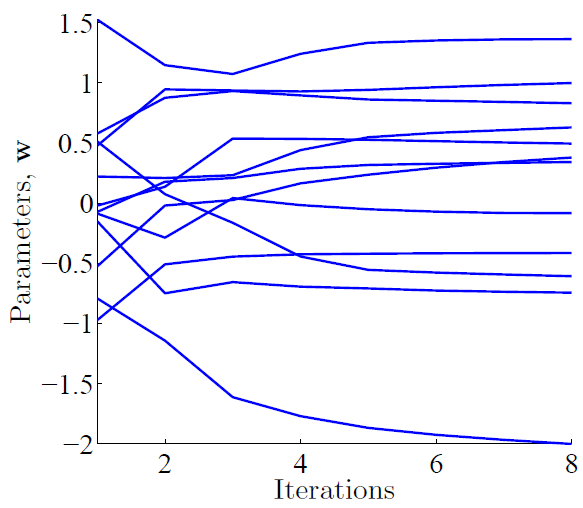
\includegraphics[width=.4\textwidth]{ConesConvPar2.png}\label{subfig:ConesConvPar2}}
\subfloat[Значение ошибки]{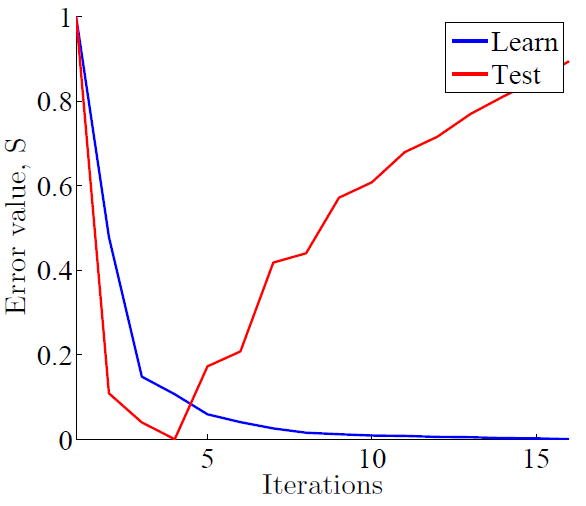
\includegraphics[width=.4\textwidth]{ConesConvErr2.png}\label{subfig:ConesConvErr2}} \\
\caption{Сходимость параметров полиэдральной модели, случай среднего количества параметров}
\label{fig:ConesConvNormal}
\end{center}
\end{figure}

\begin{figure}
\begin{center}
\subfloat[Сходимость параметров]{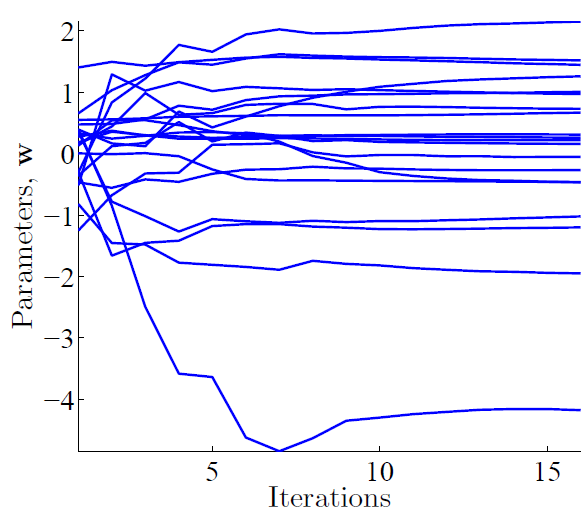
\includegraphics[width=.4\textwidth]{ConesConvPar3.png}\label{subfig:ConesConvPar3}}
\subfloat[Значение ошибки]{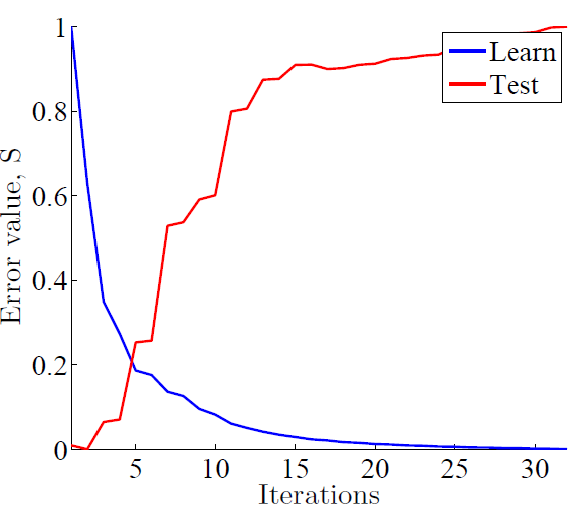
\includegraphics[width=.4\textwidth]{ConesConvErr3.png}\label{subfig:ConesConvErr3}} \\
\caption{Сходимость параметров полиэдральной модели, случай большого количества параметров}
\label{fig:ConesConvBig}
\end{center}
\end{figure}

Для иллюстрации работы алгоритма прямой оценки параметров, рассматриваемого в подразделе~\ref{subsec:ParEstDirect}, было рассмотрено три подмножества признаков различной мощности. Так, на рис.~\ref{fig:ConesConvSmall} показан случай малого количества признаков (4), на рис.~\ref{fig:ConesConvNormal}~--- среднего (12), на рис.~\ref{fig:ConesConvBig}~--- случай большого количества (все признаки). Синей линией показано значение функции ошибки на обучающей выборке, красной--- на контрольной подвыборке, выбранной случайным образом.

Видно, что в случае малого количества параметров (рис.~\ref{subfig:ConesConvErr1}) значение ошибки на обучающей и контрольной выборке монотонно уменьшается. В случае среднего количества параметров (рис.~\ref{subfig:ConesConvErr2}) значение ошибки на контроле сначала уменьшается, затем начинает расти.
На рис.~\ref{subfig:ConesConvErr3} показана сходимость функции ошибки в случае большого количества параметров. Алгоритм переобучается с первой же итерации, и ошибка на контроле начинает расти сразу. Приведенные результаты показывают необходимость применения метода снижения размерности в случае большого количества параметров.

\paragraph{Алгоритм оценивания матрицы частичного порядка.}
\begin{figure}
\begin{center}
\subfloat[Исходная матрица $\bZ_0$]{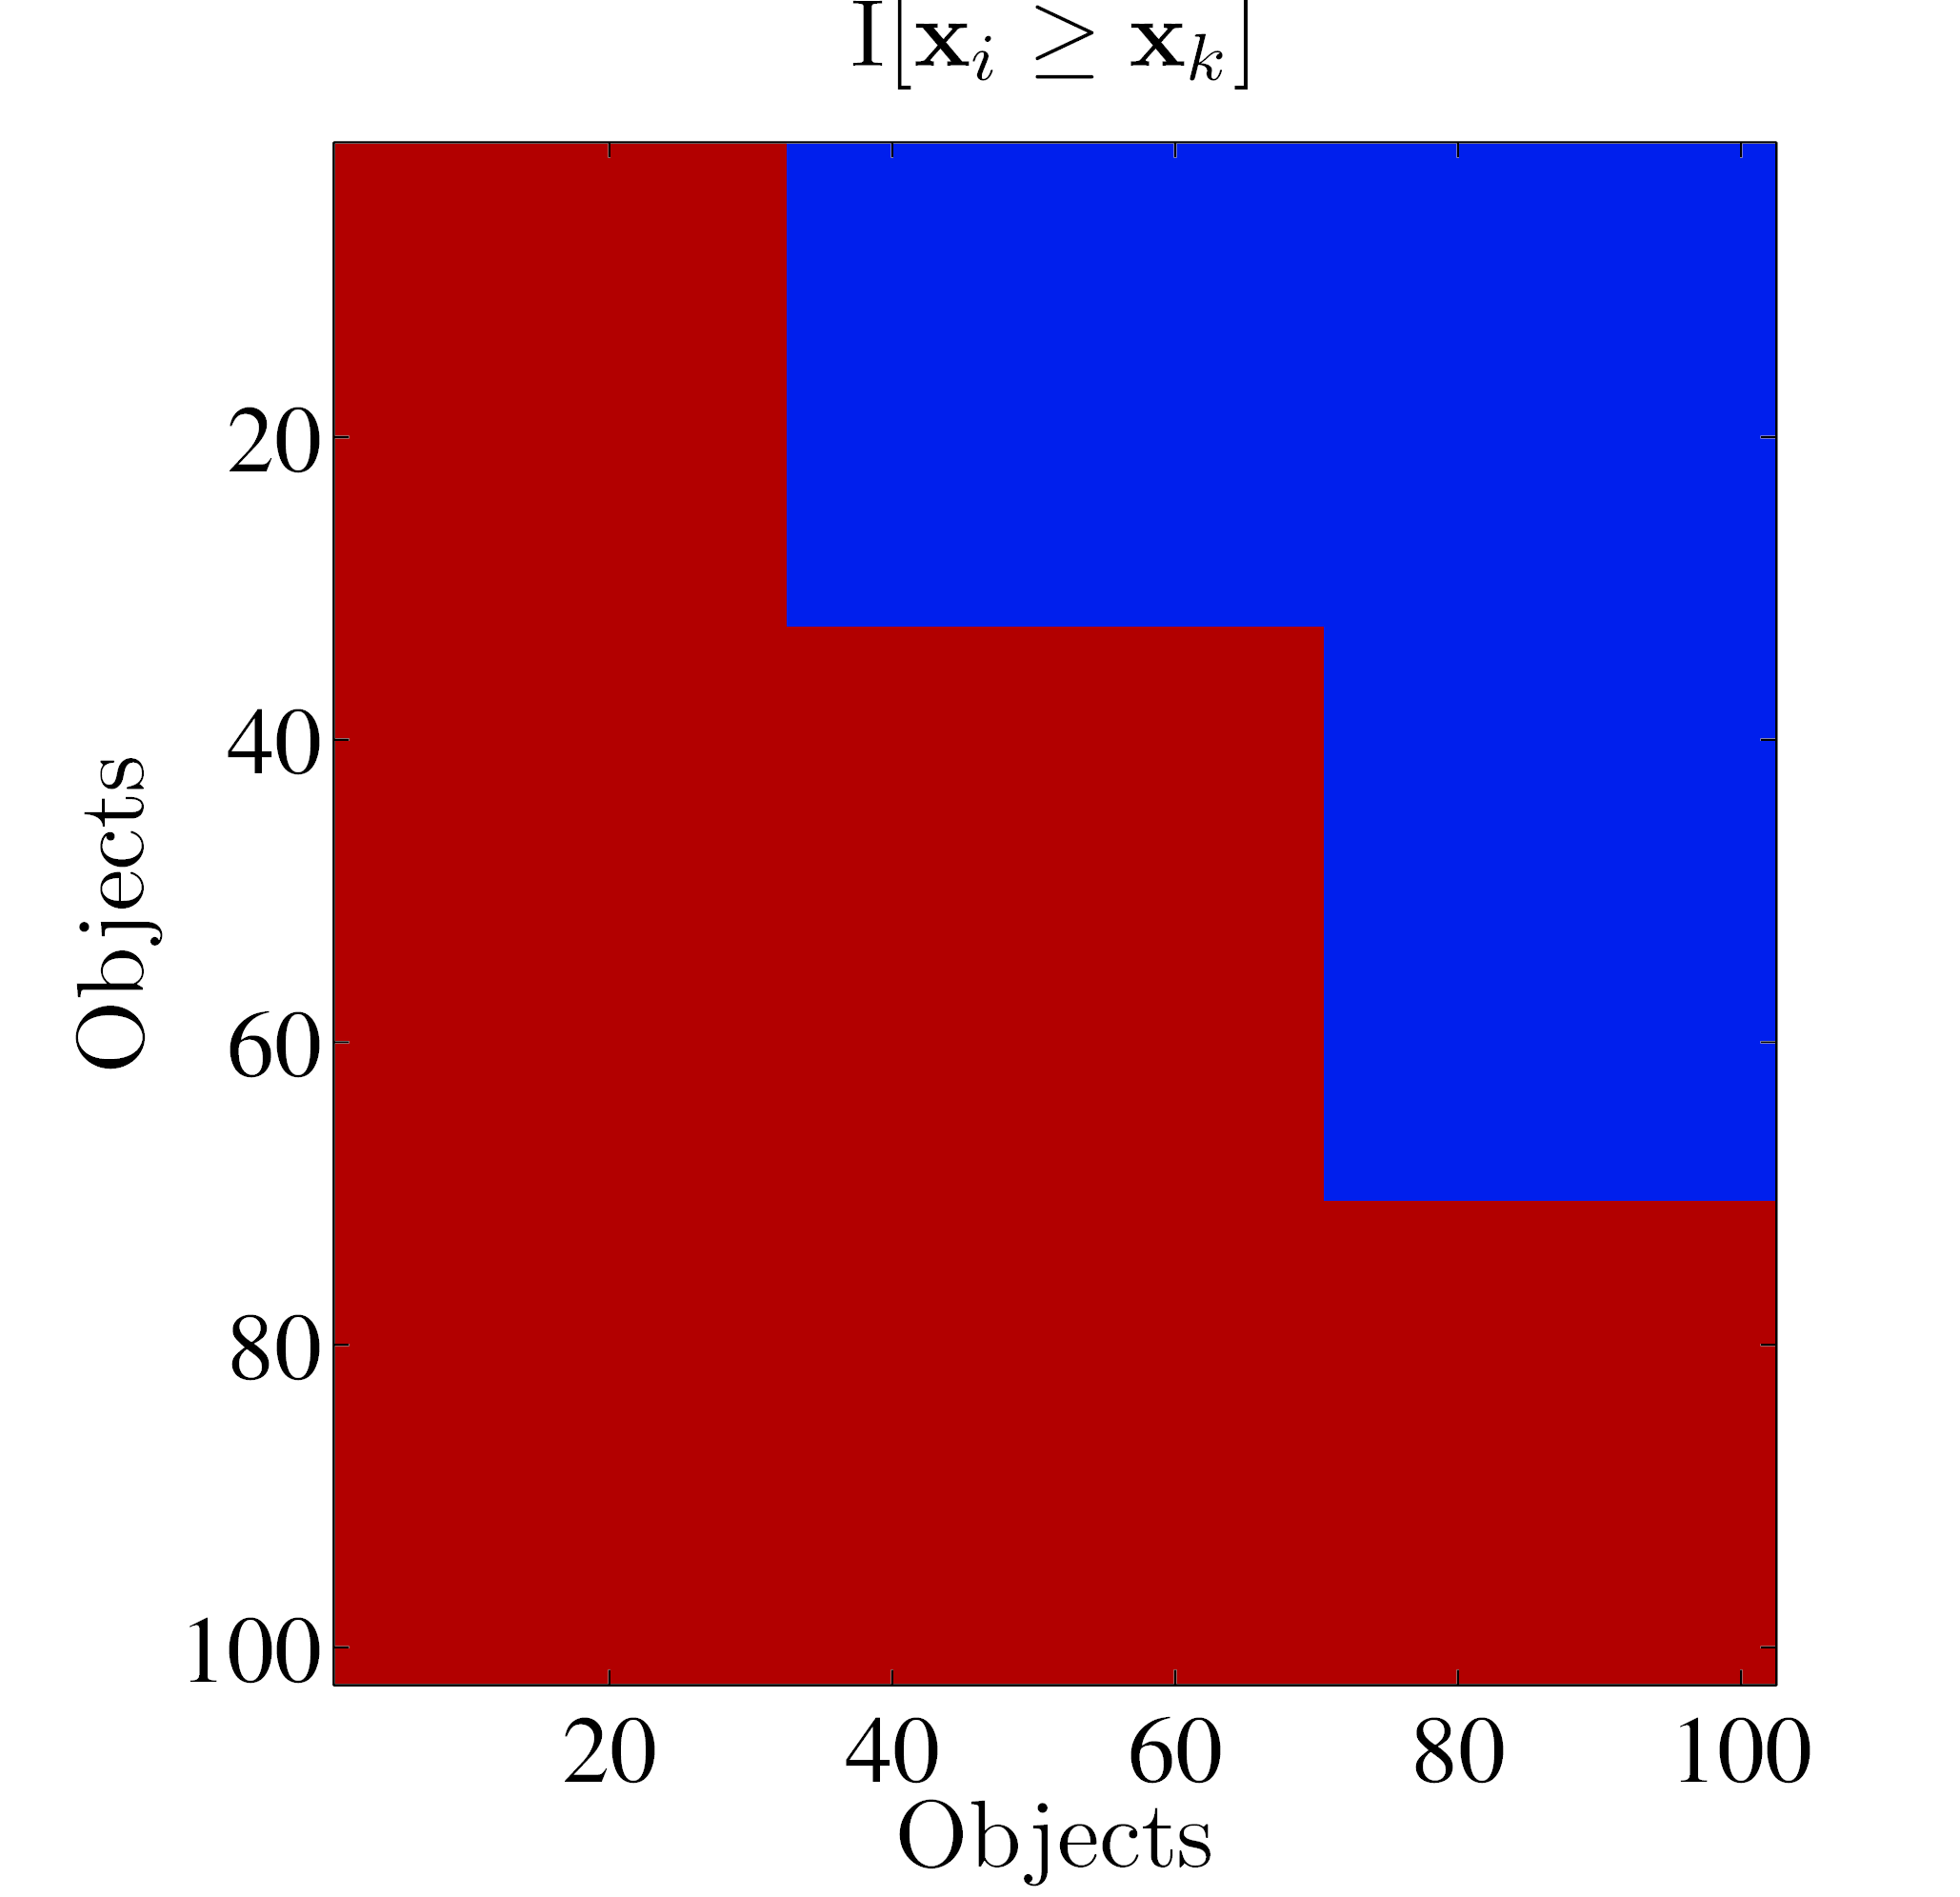
\includegraphics[width=0.49\textwidth]{Z0.png}}
\subfloat[Восстановленная матрица $\hat{\bZ}$]{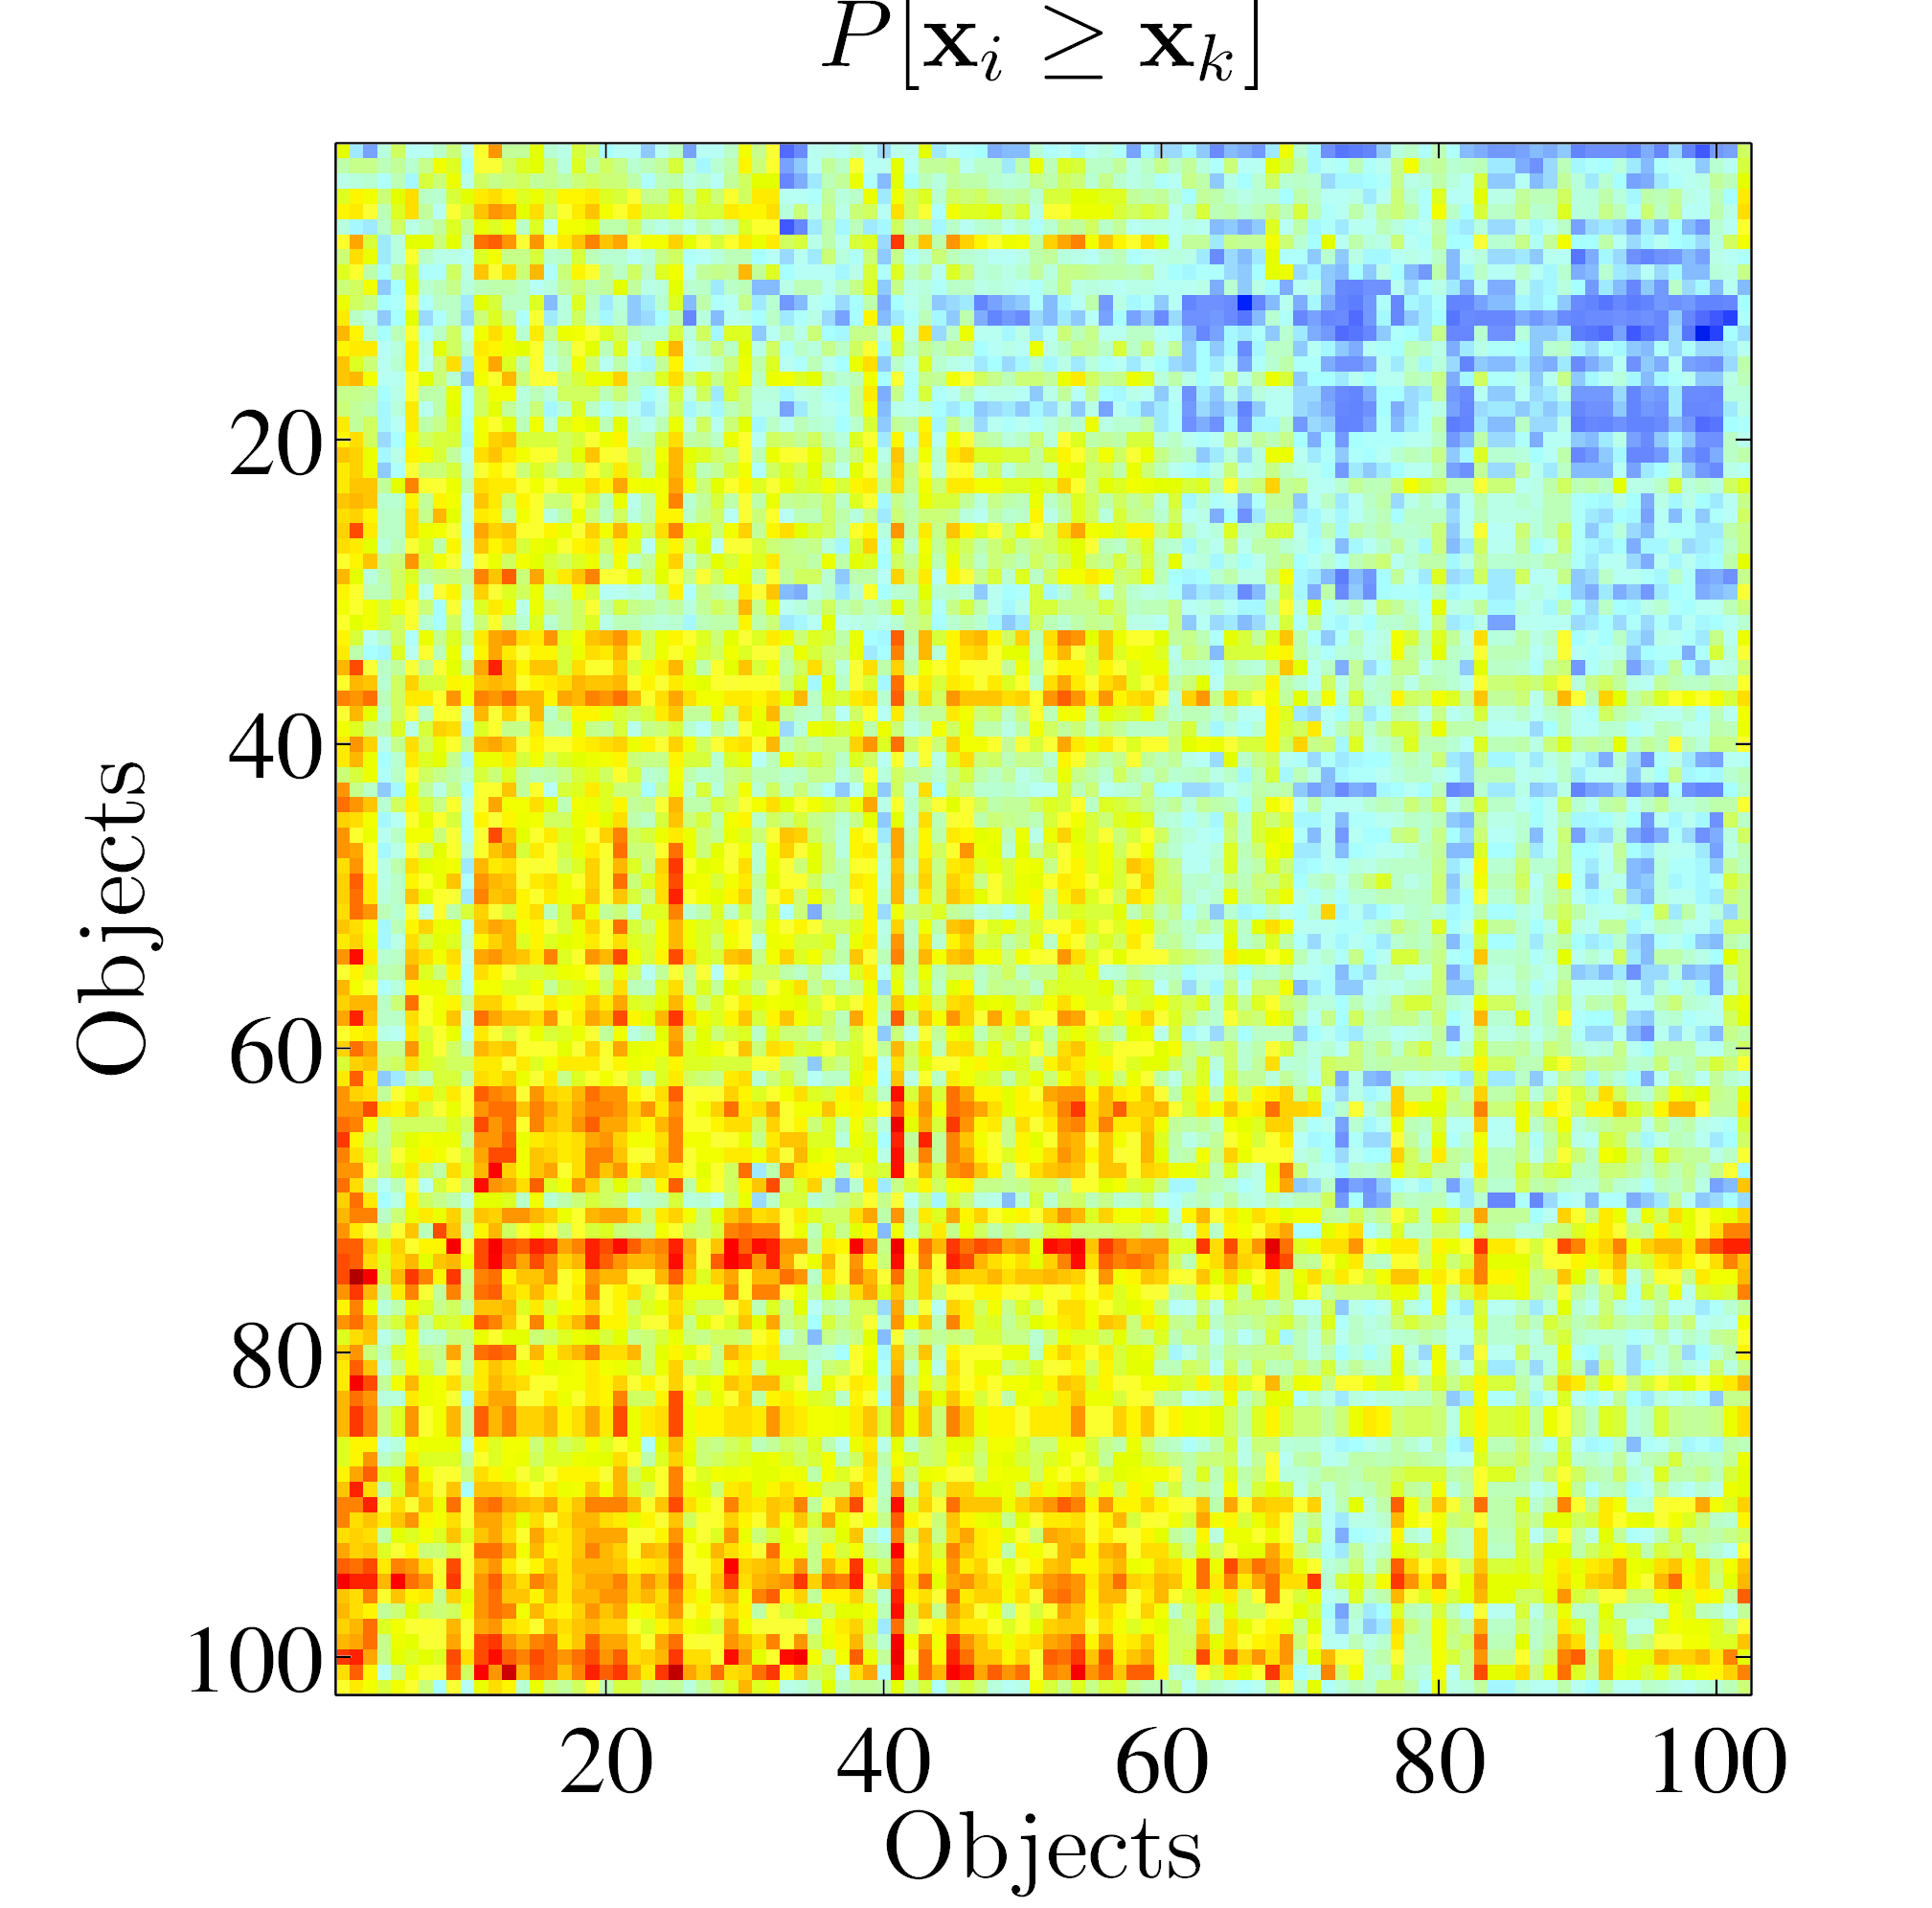
\includegraphics[width=0.49\textwidth]{Psi.png}}
\caption{Пример исходной матрицы~$\bZ_0$ и восстановленной матрицы~$\hat{\bZ}$ в задаче категоризации Красной книги}
\label{figMatrices}
\end{center}
\end{figure}
Рис.~\ref{figMatrices} иллюстрирует первый этап алгоритма из раздела~\ref{sec:PrefLearnPartMat}, оценку матрицы~$\hat{\bZ}$ по матрицам~$\bZ_0,\bZ_1,...,\bZ_n$~\eqref{eq:MatEst}.
На рис.~\ref{figMatrices} показаны исходная~$\bZ_0$ и восстановленная~$\hat{\bZ}$ матрицы для задачи категоризации Красной книги. Для этой иллюстрации выбраны объекты с тремя экспертно заданными категориями (CR --- критические, EN --- в опасности, VU --- в уязвимости), и для них построена бинарная матрица~$\bZ_0$ ступенчатого вида, соответствующая целевому отношению предпочтения~$z_0$, показанная на рис.~\ref{figMatrices}(a). На рис.~\ref{figMatrices}(b) показана восстановленная матрица~$\hat{\bZ}$. Каждый элемент матрицы~$\hat{\bZ}(i,k)$ показывает степень доминирования объекта~$\bx_k$ объектом~$\bx_i$.

\begin{figure}
\begin{center}
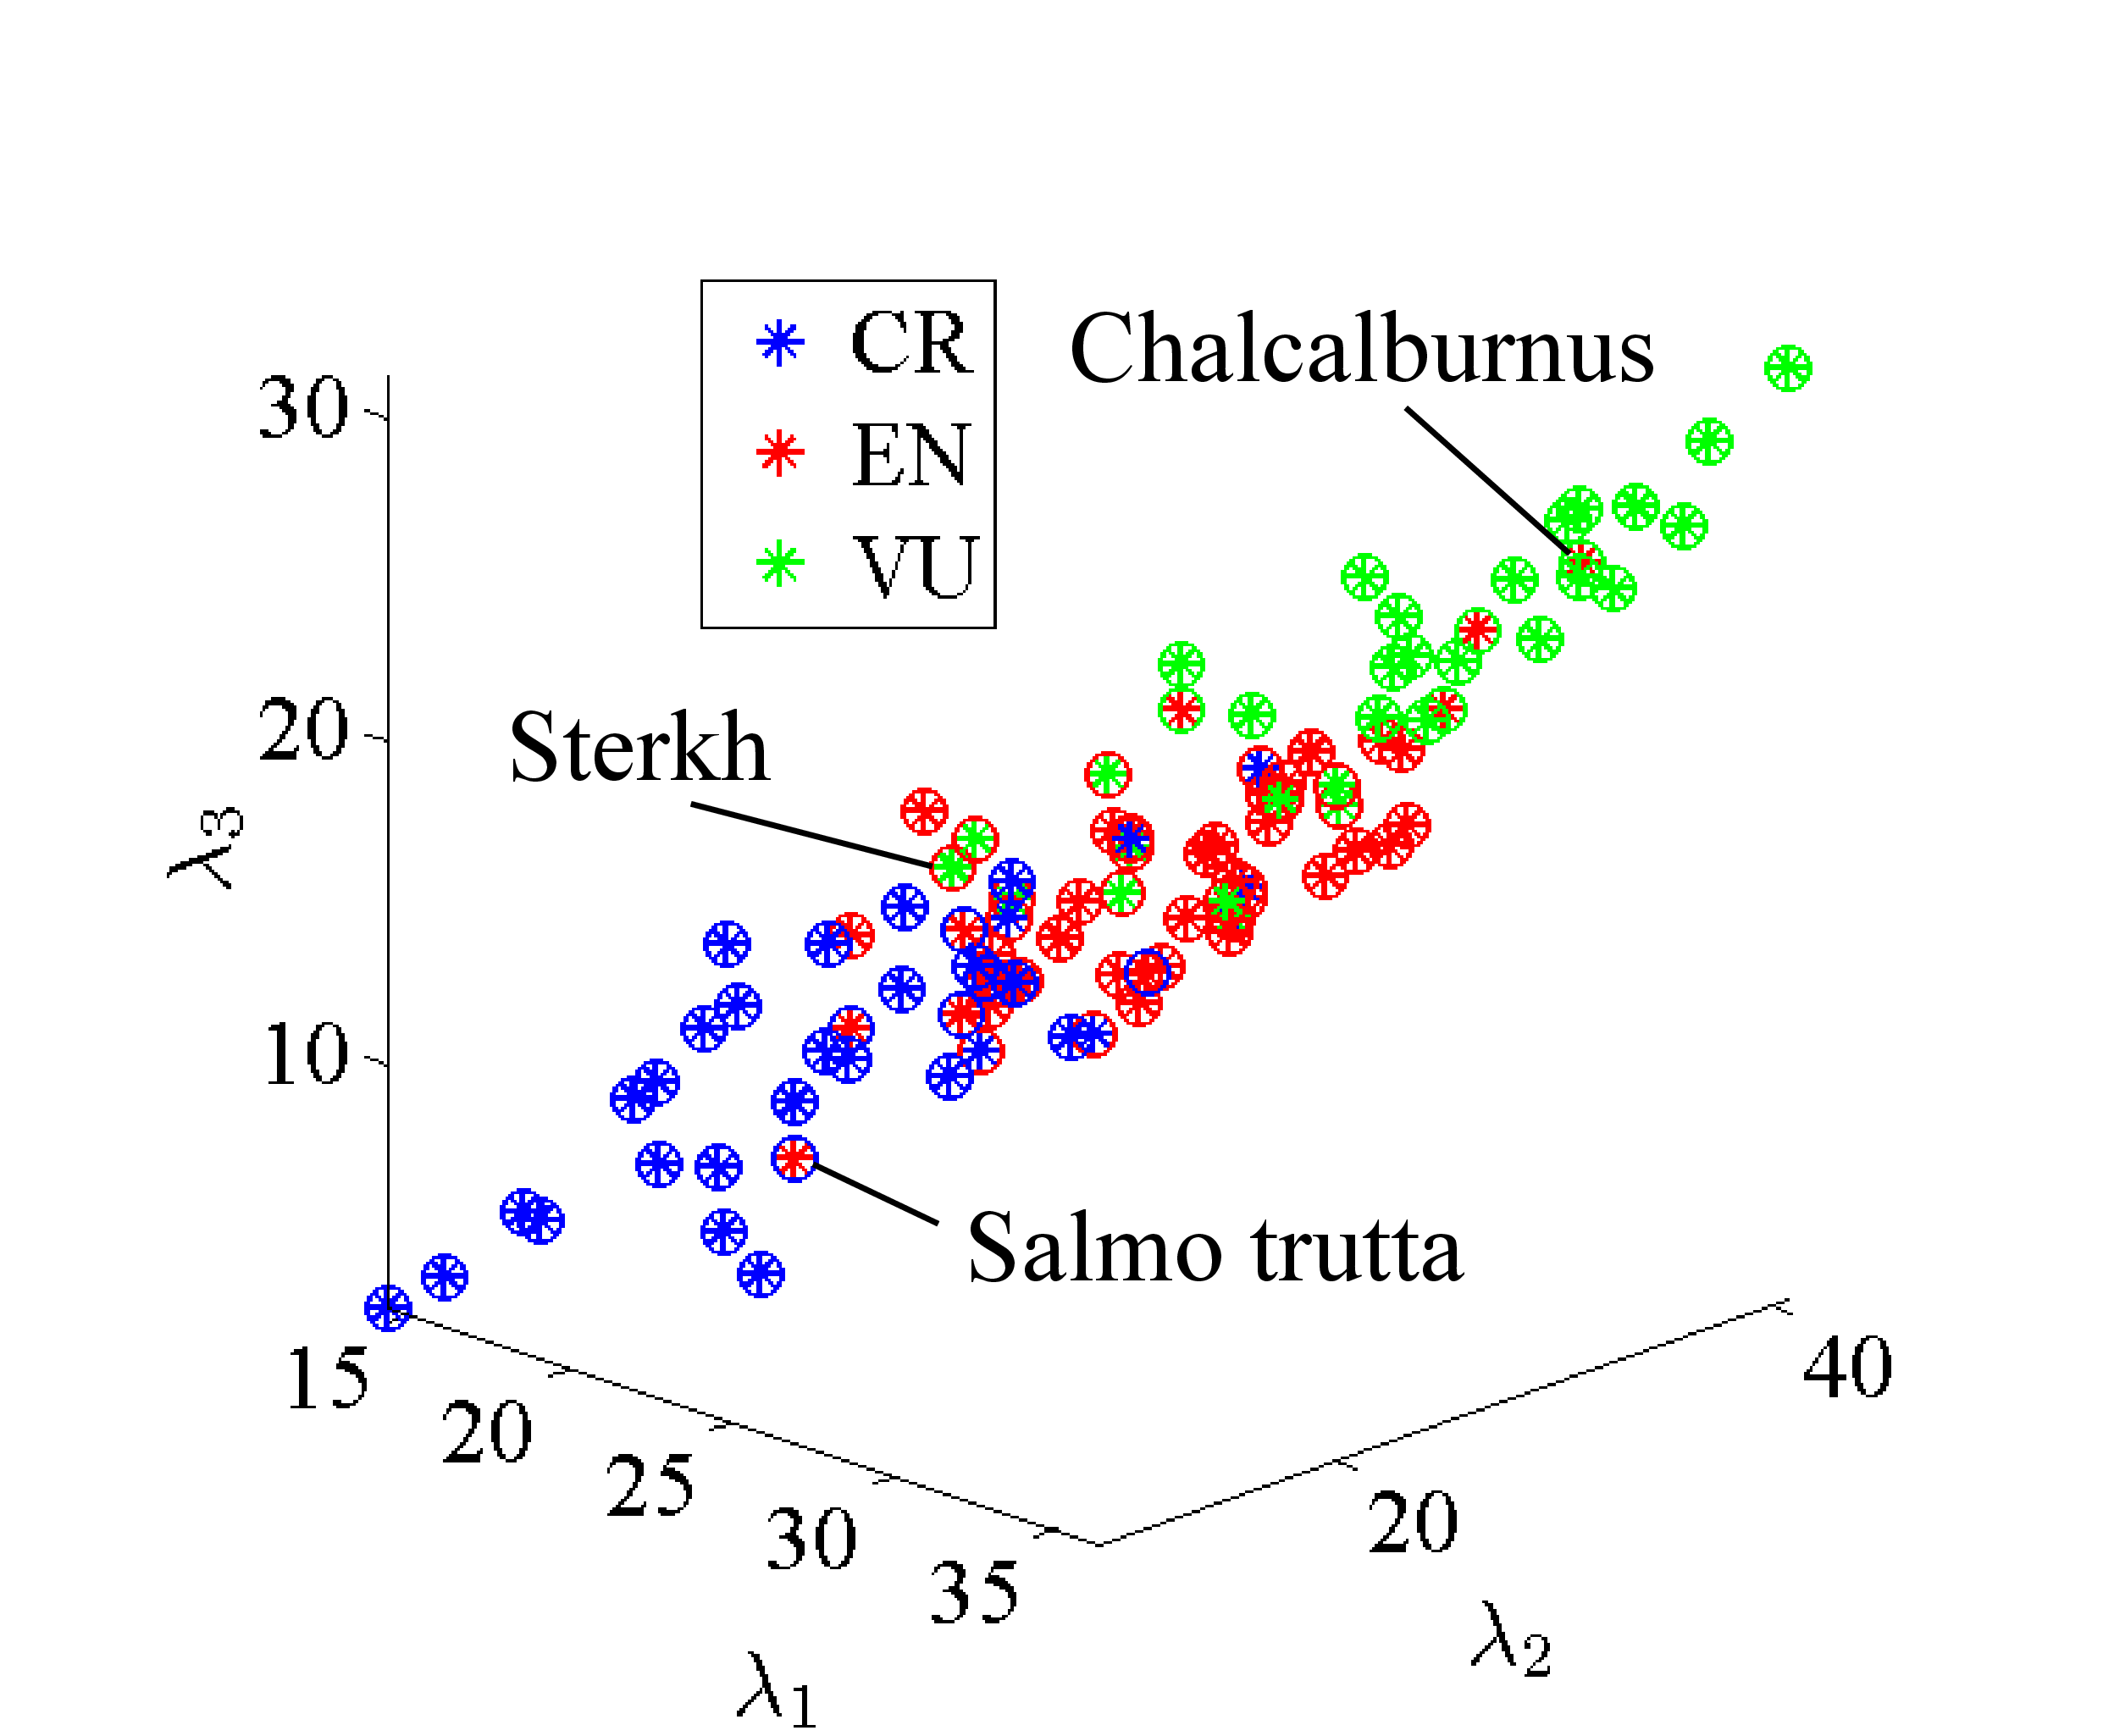
\includegraphics[width=.6\textwidth]{y1.png}
\caption{Иллюстрация классификации в задаче категоризации Красной книги}
\label{figClass}
\end{center}
\end{figure}
На рис.~\ref{figClass} показан результат работы второго этапа алгоритма для выборки из Красной книги. Для демонстрации было выбрано три столбца матрицы~$\hat{\bZ}$, поэтому пространство признаков --- трехмерное. Цвет маркера показывает исходную экспертную классификацию, цвет кружка вокруг маркера~--- классификацию, построенную алгоритмом. На рис.~\ref{figClass}, в частности, выделены объекты, отмеченные моделью как <<выбросы>>, классифицированные экспертами глубоко внутри чужого класса.

\paragraph{Сравнение алгоритмов.}
\begin{table}
%\begin{scriptsize}
\begin{center}
\caption{Категоризация Красной книги: сравнение алгоритмов}
\begin{tabular}{|c|c|}
  \hline
  Алгоритм & Средняя потеря Хэмминга \\
  \hhline{=|=}
  Матрица частичного порядка & 0.58 \\
  \hline
  Конусы & \textbf{0.52} \\
  \hline
  Копулы & 0.59 \\
  \hline
  Криволинейная регрессия & 0.71 \\
\hline
  Trees & 0.55 \\
  \hline
  SVM &  0.66 \\
  \hline
  kNN & 0.72 \\
  \hline
\end{tabular}
\label{tab:AlgComparison}
\end{center}
%\end{scriptsize}
\end{table}

В табл.~\ref{tab:AlgComparison} показано сравнение перечисленных методов. В качестве функции ошибки рассматривается средняя потеря Хэмминга~\eqref{eq:LossHamming} между метками классов на контрольной выборке. Разбиение на обучение и контроль проводилось методом leave-one-out, в таблице представлена усредненная ошибка на контрольном объекте по 102 запускам каждого алгоритма. Статистически лучший результат показал алгоритм на основе конусов из раздела~\ref{sec:PrefLearnCones}.

\subsection{Эксперименты на данных UCI}\label{sec:UCI}

Предложенные методы восстановления отношения предпочтения использованы для решения задачи порядковой классификации. Для сравнения методов были использованы наборы данных из репозитория UCI. Для того, чтобы протестировать методы на данных порядкового типа, было проведено дополнительное монотонное преобразование признаков для каждого набора данных. Проведено сравнение методов с двумя стандартными алгоритмами порядковой классификации и методом, учитывающим монотонные ограничения на признаки.

\begin{table}
%\begin{scriptsize}
\begin{center}
\caption{Описание используемых наборов данных}
\label{tab:BenchmarkData}
\begin{tabular}{cccc}
\hline
Набор данных & Признаков & Объектов & Обучение/контроль \\
\hline
Pyrimidines & 27 & 74 & 50/24 \\
MachineCPU & 6 & 209 & 150/59 \\
Boston & 13 & 506 & 300/206 \\
Computer & 21 & 8182 & 4000/4182 \\
Abalone & 8 & 4177 & 1000/3177 \\
Cars & 6 & 1728 & 1000/728 \\
RedBook & 101 & 102 & 100/1 \\
\hline
\end{tabular}
\end{center}
%\end{scriptsize}
\end{table}

Использованы следующие наборы данных из репозитория UCI: Pyrimidines, Machine CPU, Housing, Computer Activity, Abalone и Car. Перечисленные наборы данных, кроме последнего, относятся к задаче регрессии, поэтому была проведена дополнительная процедура дискретизациии целевой переменной на пять уровней, содержащих равное число объектов, для решения задачи пятиклассовой порядковой классификации.

Схема эксперимента повторяет схему из работ~\cite{stenina2015ordinal, chu2007support}. Каждый набор данных был разбит случайным образом на обучающую и контрольную части, как показано в таблице~\ref{tab:BenchmarkData}. Это разбиение было проведено независимо 100 раз. Для оценки качества были использована средняя абсолютная потеря~$L_a$,
\[
L_a(\by,\hat{\by})=\frac{1}{m}\sum\limits_{i=1}^m[y_i\neq \hat{y_i}],
\]
и средняя потеря Хэмминга~$L_H$, определяемая формулой~\eqref{eq:LossHamming}.

Было проведено сравнение алгоритма на основе взвешивания матрицы частичного порядка (OW) из раздела~\ref{sec:PrefLearnPartMat}, а также c методом классификации на основе Парето-фронтов (POF), предложенных авторами в ~\cite{stenina2015ordinal}.

Для дополнительного сравнения качества было использовано два алгоритма порядковой классификации, метод решающих деревьев (Trees) и метод опорных векторов (SVM), которые были скомбинированы со схемой порядковой классификации, описанной в~\cite{frank2001simple}. Кроме того, был использован метод классификации на основе ближайших соседей с монотонными ограничениями (KNN), описанный в~\cite{duivesteijn2008knn}.

%\begin{table}
%\begin{scriptsize}
%\begin{center}
%\caption{Результаты на данных UCI: линейные признаки}
%\label{tab:ResLinFeat}
%\begin{tabular}{|c|ccccc|ccccc|}
%\hline
%   &  \multicolumn{5}{c|}{Средняя абсолютная потеря ($\pm 0.01$)} & \multicolumn{5}{c|}{Средняя потеря Хэмминга ($\pm 0.01$)} \\
%   \hline
%Набор данных & SVM & POF & Trees & OW & KNN & SVM & POF & Trees & OW & KNN \\
%   \hhline{|=|=====|=====|}
%Pyrimidines &    \textbf{0.50}  &  0.62  &  0.61  &  0.54   & 0.55  &  \textbf{0.64}  &  0.90  &  0.84  &  0.75 &   0.75 \\
%\hline
%MachineCPU &    0.44 & 0.44 & 0.47 & \textbf{0.42} & 0.51 & 0.53 & 0.53 & 0.53 & \textbf{0.49} & 0.61 \\
%\hline
%Boston &    \textbf{0.38} & 0.48 & 0.41 & \textbf{0.39} & 0.47 & \textbf{0.46} & 0.65 & \textbf{0.47} & \textbf{0.46} & 0.62 \\
%\hline
%Computer &    \textbf{0.32} & 0.71 & 0.38 & 0.34 & 0.60 & \textbf{0.35} & 1.36 & 0.41 & 0.39 & 0.90 \\
%\hline
%Abalone &    \textbf{0.53} & 0.59 & 0.57 & 0.56 & 0.60 & \textbf{0.78} & 0.92 & \textbf{0.77} & 0.81 & 0.88 \\
%\hline
%\end{tabular}
%\end{center}
%\end{scriptsize}
%\end{table}
%
%Результаты для пяти искомых наборов данных (всех перечисленных, кроме <<Cars>>) представлены в таблице~\ref{tab:ResLinFeat}. Жирным выделены случаи, когда соответствующий алгоритм показал статистически лучший результат по сравнению с остальными для 100 разбиений данных. Видно, что хотя метод SVM  превосходит остальные методы из-за линейной природы признаков, тем не менее, предложенный метод OW срабатывает лучше на наборах данных MachineCPU и Boston.

\begin{table}
\begin{scriptsize}
\begin{center}
\caption{Результаты на данных UCI: порядковые признаки}
\label{tab:ResOrdFeat}
\begin{tabular}{|c|ccccc|ccccc|}
\hline
   &  \multicolumn{5}{c|}{Средняя абсолютная потеря ($\pm 0.01$)} & \multicolumn{5}{c|}{Средняя потеря Хэмминга ($\pm 0.01$)} \\
   \hline
Набор данных & SVM & POF & Trees & OW & KNN & SVM & POF & Trees & OW & KNN \\
   \hhline{|=|=====|=====|}
Pyrimidines &    0.57 & 0.58 & 0.60 & 0.62 & \textbf{0.49} & \textbf{0.71} & 0.77 & 0.79 & 0.79 & 0.76 \\
\hline
MachineCPU &    0.51 & \textbf{0.39} & 0.47 & \textbf{0.40} & 0.43 & 0.65 & \textbf{0.45} & 0.56 & 0.47 & 0.51 \\
\hline
Boston &     \textbf{0.40} & 0.48 & \textbf{0.40} & 0.43 & \textbf{0.41} & 0.49 & 0.68 & \textbf{0.46} & 0.50 & 0.51 \\
\hline
Computer &     0.44 & 0.69 & 0.41 & \textbf{0.37} & 0.45 & 0.53 & 1.38 & \textbf{0.45} & \textbf{0.44} & 0.55 \\
\hline
Abalone &    0.78 & \textbf{0.59} & \textbf{0.57} & \textbf{0.58} & \textbf{0.59} & 1.78 & 0.92 & \textbf{0.76} & 0.85 & 0.89 \\
\hhline{|=|=====|=====|}
Cars &    0.19 & 0.19 & 0.08 & 0.16 & \textbf{0.06} & 0.24 & 0.26 & \textbf{0.08} & 0.19 & \textbf{0.07} \\
\hline
RedBook &    0.56 & 0.61 & \textbf{0.50} & \textbf{0.49} & 0.59 & 0.66 & 0.74 & \textbf{0.55} & 0.59 & 0.72 \\
\hline
\end{tabular}
\end{center}
\end{scriptsize}
\end{table}

Для сравнения методов на данных порядковой природы была произведена порядковая трансформация признаков исходных наборов данных. Также, как и в случае с целевой переменной, была произведена дискретизация каждого признака на пять уровней, содержащих одинаковое количество объектов.

Результаты для преобразованных наборов данных, а также для набора <<Cars>>, признаки которого изначально имели порядковую природу, показаны в таблице~\ref{tab:ResOrdFeat}. Метод SVM для данных такого типа сработал значительно хуже, а методы Trees и KNN показали лучший результат. Рассматриваемый метод OW продемонстрировал лучший результат в терминах средней абсолютной потери.

Результаты тестирования для задачи категоризации Красной книги показаны в последней строке таблицы~\ref{tab:ResOrdFeat}. В отличие от остальных наборов данных, для этой задачи была использована схема разбиения leave-one-out, как и в подразделе~\ref{sec:IUCN}. Предложенный метод продемонстрировал наилучший результат наряду с методом Trees.

\section{Заключение}
Разработан новый подход к построению математической модели предпочтений на основе полиэдрального представления порядковых данных. Разработаны новые вычислительные методы агрегирования порядковых признаков, основывающиеся на построении суперпозиции конусов предпочтений. Показано, что предлагаемая модель является обобщением модели порядковой классификации с монотонными ограничениями. Установлено теоретическое соответствие между конусом и матрицей инцидентности графа предпочтений. Проведено обобщение известных порядковых метрик на случай частичных порядков с использованием матрицы предпочтений.

%В работе устанавливаются теоретические обобщения ранее полученных результатов в области обучения по предпочтениям путем введения понятия конуса предпочтений. Введенные понятия обобщают понятия ранговой корреляции и монотонных ограничений.

Приведено решение задачи категоризации редких видов из Красной книги РФ. Проведено сравнение разработанных методов для решения задачи порядковой классификации на стандартных наборах данных из репозитория UCI. Разработанные методы показывают улучшение качества в сравнении с известными подходами.

%\section{Аппендикс}
%В этом разделе приведем некоторые свойства отношений предпочтения. В частности, выразим в терминах матрицы предпочтений некоторые порядковые метрики (ранговую корреляцию Спирмена, Кендалла), правило Кемени, а также характеристику площади под кривой (AUC). Приведенные обобщения порядковых метрик будут использоваться в последующих разделах в качестве оптимизируемых функций потерь.
%
%\paragraph{Ранговая корреляция.} Пусть задано множество объектов~$X=\{x_1,....,x_m\}$, и на этом множестве задано два различных отношения предпочтения, выраженных отношениями частичного порядка~$z_1,z_2$. Ниже введем два известных определения корреляции Спирмена и Кендалла между двумя векторами рангов, определенных на множестве~$X$.
%
%\begin{df}
%Коэффициентом корреляции Спирмена~$\rho_s$ называется величина
%\[
%\rho_s=1-\frac{6}{m(m-1)(m+1)}\sum\limits_{i=1}^m(R_i-S_i)^2,
%\]
%где~$R_i$--- ранг объекта~$x_i$ во множестве~$X$ согласно отношению~$z_1$, $S_i$--- ранг объекта~$x_i$ во множестве~$X$ согласно отношению~$z_2$.
%\end{df}
%
%\begin{lemm}
%Для коэффициента корреляции Спирмена выполнено следующее соотношение:
%\begin{equation}
%\rho_s\propto -\sum\limits_{i=1}^m\left(\sum\limits_{k=1}^m(\bZ_1(i,k)-\bZ_2(i,k))\right)^2,
%\label{eq:SpearZ}
%\end{equation}
%где~$\bZ_1,\bZ_2$~--- матрицы предпочтений, соответствующих~$z_1,z_2$.
%\end{lemm}
%\begin{proof}
%Доказательство этой леммы следует из того факта, что ранг наблюдения объекта~$x_i$ является суммой значений всех элементов матрицы~$\bZ$ в строке~$i$.
%\end{proof}
%\begin{df}
%Коэффициентом корреляции Кендалла~$\tau$ называется величина, подсчитывающая количество инверсий в двух порядковых рядах:
%\[
%\tau=1-\frac{4}{m(m-1)}R,~~\text{где}~~R=\sum\limits_{i=1}^{m-1}\sum\limits_{k=1}^m I\left[z_1(x_i,x_k) \neq z_2(x_i,x_k)\right].
%\]
%\end{df}
%\begin{lemm}
%Для коэффициента корреляции Кендалла справедливо соотношение:
%\begin{equation}
%\tau\propto -\sum\limits_{i=1}^m\sum\limits_{k=1}^m(\bZ_1(i,k)-\bZ_2(i,k))^2=-\|\bZ_1-\bZ_2\|_F,
%\label{eq:KendZ}
%\end{equation}
%где~$\|\cdot\|_F$~--- норма Фробениуса.
%\end{lemm}
%Доказательство этой леммы следует непосредственно из определения корреляции Кендалла.
%
%Отметим, что формулы~\eqref{eq:SpearZ} и~\eqref{eq:KendZ} позволяют обобщить стандартные ранговые корреляции Спирмена и Кендалла на случай частичных порядков, а также на случай нечеткого отношения предпочтения~$\bZ(i,k)\in [0,1]$, который будет рассмотрен в дальнейшем.
%
%\paragraph{Медиана Кемени.} Согласно формуле~\eqref{eq:KemenyRule}, правило Кемени заключается в поиске линейного порядка~$z$ на множестве объектов~$X$, являющегося средним в смысле $\tau$-корреляции для всех порядков~$z_1,...,z_n$, определенных на~$X$. Из формулы~\eqref{eq:KendZ} непосредственно следует лемма об обобщении правила Кемени на случай частичных порядков, задаваемых матрицами~$\bZ_i$.
%
%\begin{lemm}
%Медианой в смысле Кемени называется линейный порядок, задаваемый матрицей~$\bZ^*$, минимизирующей выражение
%\[
%\bZ^*=\arg\min\limits_{\bZ\in \text{LO}}\sum\limits_{i=1}^n\|\bZ-\bZ_i\|_F,
%\]
%где $\text{LO}$~--- множество матриц, задающих линейный порядок.
%\end{lemm}
%
%\paragraph{Площадь под кривой.} Используем понятие матрицы предпочтений для обобщения понятия площади под кривой (Area Under Curve, AUC), используемый для измерения качества алгоритма классификации, на случай задачи многоклассовой порядковой классификации.
%
%Рассмотрим исходную формулу вычисления AUC для случая двух классов. Задано множество пар объект-ответ~$\{(x_1,y_1),...,(x_m,y_m)\}$, где $y_i \in \{0,1\}$. Обозначим за~$m_0$ количество объектов класса 0, а за~$m_1$~--- количество объектов класса 1. За вектор~$\mathbf{p}$ обозначим вектор ответов алгоритма классификации размера~$m$, $p_i\in \mathbb{R}$. В этом случае, площадь под кривой вычисляется по формуле
%\begin{equation}
%\text{AUC}=\frac{1}{m_0m_1}\sum\limits_{k=1}^{m_0}\sum\limits_{i=1}^{m_1} [p_i>p_k].
%\label{eq:AucBase}
%\end{equation}
%
%Из определения матрицы предпочтения следует утверждение о представлении AUC:
%\begin{lemm}
%\begin{equation}
%\text{AUC}=\frac{1}{m_0m_1}\sum\limits_{k,i=1}^{m} [\bZ(k,i)=0][\hat{\bZ}(k,i)=0],
%\label{eq:AucZ}
%\end{equation}
%где~$\hat{\bZ}$~--- матрица предпочтений, соответствующая вектору оценок алгоритма~$\mathbf{p}$.
%\end{lemm}
%\begin{proof}
%Формула~\eqref{eq:AucZ} может быть переписана в виде
%\[
%\text{AUC}=\frac{1}{m_0m_1}\sum\limits_{k,i=1}^{m}[y_k=0,y_i=1][p_k<p_i]=\frac{1}{m_0m_1}\sum\limits_{i=1}^{m_0}\sum\limits_{k=1}^{m_1} [p_i>p_k].
%\]
%\end{proof}
%
%Обобщим понятие площади под кривой на многоклассовый порядковый случай с использованием матрицы предпочтений. Пусть~$Y$ является конечным множеством меток,~$Y=\{1,...,K\}$ с соответствующим количеством элементов в выборке~$m_1,...,m_k$. Формула~\eqref{eq:AucZ} обобщается следующим образом:
%\begin{equation}
%\text{AUC}=\frac{1}{M}\sum\limits_{k,i=1}^{m} [\bZ(k,i)=0][\hat{\bZ}(k,i)=0],
%\label{eq:AucMult}
%\end{equation}
%где~$M=\sum\limits_{k_1\prec k_2}m_{k_1}m_{k_2}$. Отметим, что в двуклассовом случае многоклассовая формула~\eqref{eq:AucMult} переходит в~\eqref{eq:AucZ}. Кроме того, для задачи регрессии, когда~$y=\mathbb{R}$, справедливо следующее утверждение.
%\begin{lemm}
%В случае задачи регрессии, AUC, определенный формулой~\eqref{eq:AucMult}, равен $\tau$-корреляции между вектором ответов и вектором оценок алгоритма.
%\end{lemm}
%\begin{proof}
%В случае задачи регрессии,~$M=m(m-1)/2$ и
%\[
%\begin{split}
%\text{AUC}=\frac{2}{m(m-1)}\sum\limits_{k,i=1}^{m} [\bZ(k,i)=0][\hat{\bZ}(k,i)=0]=\frac{2}{m(m-1)}\sum\limits_{k,i=1}^{m}[y_k<y_i][p_k<p_i]= \\
%= 1 - \frac{4}{m(m-1)}\sum\limits_{i=1}^{m-1}\sum\limits_{k=i+1}^{m}\left[[y_k<y_i]\neq[p_k<p_i]\right]=\tau(\by,\mathbf{p}).
%\end{split}
%\]
%\end{proof}

\bibliographystyle{plain}
\bibliography{KuznetsovPreferenceLearning}

\end{document}
